% ============================================================================
% 第 5 章  拉格朗日 Floer（上）同调  （原书 pp.63–84，PDF pp.66–87）
% ============================================================================
\section{拉格朗日 Floer（上）同调}\label{ch:05}

% 原书公式在全书范围内连续编号，本章从 (54) 起到 (77) 止，共 24 个编号公式。
% 此处把计数器设为 53，使本章第一个 equation 环境自动编为 (54)，与原文逐号对应。
\setcounter{equation}{53}

\takeaway{%
  核心图像：拉格朗日 Floer 上同调是两条拉格朗日子流形交点上的“无穷维 Morse 理论”，
  其微分由 $J$-全纯条带的计数给出。\\
  数学工具：辛几何与近复几何、Maslov 指标与分次、伪全纯曲线模空间的横截性、
  紧致性与可定向性、Novikov 域。\\
  主要结论：在 $2c_1(TM)=0$、消没 Maslov 类与“无冒泡”条件下，$\partial^2=0$，
  $HF(L_0,L_1)$ 与微扰数据 $(J,H)$ 的选取无关，且 $HF(L,L)\cong H(L;\Lambda_{\mathbb K})$；
  在正合流形情形，形式变量 $T$ 可被消去，直接在域 $\mathbb K$ 上工作。%
}

\subsection{辛几何与复几何预备}\label{sec:5.1}

本节以简短而略显紧凑的方式，介绍 Fukaya 范畴理论所依赖的全部几何概念。
先从辛几何这一分支谈起（更详细的内容可参阅 \cite{Sil12}）。

\begin{Def}\label{def:5.1}
一个 $2n$ 维\emph{辛流形} $(M,\omega)$ 是光滑流形 $M^{2n}$ 连同\emph{辛形式}
$\omega\in\Omega^2(M)=\Gamma(\Lambda^2(T^*M))$，即一个闭的非退化 $2$-形式
（于是对每个 $x\in M$，它典范地给出反对称双线性映射
$\omega_x:T_xM\times T_xM\to\mathbb R$，使得若 $\omega_x(v,w)=0$ 对所有
$w\in T_xM$ 成立，则 $v=0\in T_xM$）。\emph{闭性}指 $d\omega=0$，其中
$d:\Omega^\bullet(M)\to\Omega^{\bullet+1}(M)$ 为外微分算子。

若 $\omega$ 是正合 $2$-形式，即存在某个 $\nu\in\Omega^1(M)$ 使 $\omega=d\nu$，
则称 $M$ 是\emph{正合的}。当 $M$ 紧致时，可以证明 $\omega$ 绝不可能正合，
也就是说 $\langle\omega\rangle\in H^2_{\mathrm{dR}}(M)$ 是 de Rham 上同调中的
非平凡类。
\end{Def}

% [Tutor Note: 【背景】非退化交替双线性形式只存在于偶数维：若再加闭性，则
% $\omega^n$ 处处非零、给出 $M$ 的一个体积形式，故 $M$ 自动可定向；这正是原文
% “$\omega$ 的定义本身迫使 $M$ 为偶数维且可定向”的全部内容。]

我们注意，$\omega$ 的定义本身迫使 $M$ 为偶数维且可定向。

\begin{Def}\label{def:5.2}
设 $(M,\omega)$ 是 $2n$ 维辛流形。$M$ 的\emph{拉格朗日子流形} $L\subset M$
是 $M$ 的极大迷向子流形，即维数为 $\frac12\dim(M)=n$ 且满足 $\omega|_L=0$
的子流形（等价地，对包含映射 $\iota:L\hookrightarrow M$ 有 $\iota^*\omega=0$）。

假设 $M$ 正合，$\omega=d\nu$，其中 $\nu\in\Omega^1(M)$。若限制 $\nu|_L$
（它是闭的，因为 $d(\nu|_L)=(d\nu)|_L=0$）是正合 $1$-形式，即存在某个光滑函数
$f\in C^\infty(L)$ 使 $\nu|_L=df$，则称 $L$ 本身是\emph{正合的}。
\end{Def}

\begin{Rem}\label{rem:5.3}
作为特例，向量空间 $V$ 若配有反对称非退化映射 $\omega:V\times V\to\mathbb R$
（称为\emph{辛结构}），则称为\emph{辛向量空间}。此时线性子空间 $W\subset V$
是\emph{拉格朗日的}，若 $W=W^\perp:=\{v\in V\mid \omega(v,w)=0\ \forall w\in W\}$。
这是\emph{拉格朗日 Grassmann 流形}
$LGr(V):=\{W\subset V\mid W\ \text{为线性拉格朗日子空间}\}$ 的一个元素；
$LGr(V)$ 是光滑流形，微分同胚地可实现为齐性空间 $U(n)/O(n)$
（酉矩阵模正交矩阵）。

例如，在 $V:=\mathbb R^{2n}$ 上取 $\omega_0\in\Omega^2(\mathbb R^{2n})$，它由矩阵
$\bigl(\begin{smallmatrix}0&\mathbf 1_n\\ 1_n&0\end{smallmatrix}\bigr)$
表示；则子空间 $W\subset\mathbb R^{2n}$ 是拉格朗日的当且仅当它是 $n$ 维的，
且 $\omega_0((x_1,y_1),(x_2,y_2)):=x_1\cdot y_2-x_2\cdot y_1=0$ 对所有
$(x_1,y_1),(x_2,y_2)\in W$ 成立。此时我们干脆写 $LGr(n)$ 代替
$LGr(\mathbb R^{2n})$。再回忆辛群
\[
\operatorname{Sp}(2n,\mathbb R)=\{B\in\operatorname{GL}(2n,\mathbb R)\mid
\omega_0(B(v),B(w))=\omega_0(v,w)\ \forall v,w\in\mathbb R^{2n}\}
\equiv\{B\in\mathbb R^{2n\times2n}\mid B^T\omega_0B=\omega_0^T\}.
\]

% [Tutor Note: 【勘误】原文把辛群的条件印作 $B^T\omega_0B=\omega_0^T$；按
% $\operatorname{Sp}$ 的定义应为 $B^T\omega_0B=\omega_0$（因
% $\omega_0^T=-\omega_0$，两式相差一个符号）。译文照印，读者引用时以
% $B^T\omega_0B=\omega_0$ 为准。]

显然，若 $(M^{2n},\omega)$ 是辛流形，则 $(T_xM,\omega_x)$ 是辛向量空间，
且对每个 $x\in M$ 有 $LGr(T_xM)\cong LGr(n)$（我们说向量丛 $TM\to M$ 是
\emph{辛的}）。对拉格朗日子流形 $L^n$ 的任一点 $x\in L$，按定义有
$T_xL\in LGr(T_xM)$。
\end{Rem}

我们还要回顾哈密顿动力学的基本内容。

\begin{Def}\label{def:5.4}
设 $(M,\omega)$ 是辛流形。对每个光滑函数 $H\in C^\infty(M)$，可对应一个向量场
$X_H\in\mathfrak X(M)$，满足 $i_{X_H}(\omega)=\omega(\,\cdot\,,X_H)=dH:
\mathfrak X(M)\to C^\infty(M)$。$X_H$ 称为与\emph{哈密顿函数} $H$ 相伴的
\emph{哈密顿向量场}。
\end{Def}

若哈密顿量依赖时间，$H\in C^\infty(I\times M)$，其中
$H(t,\,\cdot\,)\equiv H_t(\,\cdot\,)\in C^\infty(M)$ 且 $I=[0,1]$（或
$\mathbb R$），则它给出一族哈密顿向量场 $\{X_{H_t}\}_{t\in I}\subset\mathfrak X(M)$；
对 $X_H$（假定完备）可对应其哈密顿“流” $\phi_H:I\times M\to M$，满足
\[
\frac{d}{dt}\Big|_t(\phi_H^t)=X_{H_t}\circ\phi_H^t
\quad\text{且}\quad \phi_H^0=\mathrm{id}
\]
（我们写 $\phi_H(t,\,\cdot\,)=\phi_H^t(\,\cdot\,)$）。特别地，称 $\phi_H^1$ 为
$H$ 生成的\emph{哈密顿微分同胚}。它是群
\[
\operatorname{Ham}(M,\omega):=\{\phi\in\operatorname{Diff}(M)\mid
\phi=\phi_H^1\ \text{为某个}\ H\in C^\infty(I\times M)\ \text{的哈密顿微分同胚}\}
\]
的一个元素。记 $\operatorname{Symp}(M,\omega):=\{\phi\in\operatorname{Diff}(M)\mid
\phi^*\omega=\omega\}$ 为辛同胚群，则有子群的包含关系
\[
\operatorname{Ham}(M,\omega)\le\operatorname{Symp}(M,\omega)\le
\operatorname{Diff}(M).
\]

\begin{Def}\label{def:5.5}
设 $M$ 是光滑流形，$L_0,L_1\subset M$ 是紧致子流形。
\begin{itemize}
  \item 称 $L_0$ 与 $L_1$ \emph{横截相交}（或\emph{横截}），若
  $T_xL_0\pitchfork T_xL_1$，即作为向量空间
  $T_xL_0\oplus T_xL_1=T_xM$ 对所有 $x\in L_0\cap L_1\subset M$ 成立。
  此时记 $L_0\pitchfork L_1$。
  \item $L_0$ 与 $L_1$ 之间的（光滑）\emph{同痕}是一个紧子流形
  $\widetilde L\subset M\times[0,1]$，使得
  $\widetilde L\cap(M\times\{i\})=L_i\times\{i\}$（$i=0,1$），且
  $\widetilde L\pitchfork(M\times\{t\})$ 对所有 $t\in[0,1]$ 成立。
  此时 $L_0$ 与 $L_1$ 也是\emph{环境同痕的}，即存在道路
  $\phi:t\in[0,1]\mapsto\phi_t\in\operatorname{Diff}(M)$ 使
  $\phi_0=\mathrm{id}_M$ 且 $\phi_1(L_0)=L_1$。
  \item 现在设 $M=(M,\omega)$ 还是辛流形且 $L_0,L_1$ 拉格朗日。上述同痕
  $\widetilde L$ 是\emph{拉格朗日同痕}，若此外每个
  $\widetilde L\cap(M\times\{t\})\subset M\times\{t\}$ 是拉格朗日子流形；
  由此推出 $(\pi_1^*\omega)|_{\widetilde L}=\theta\wedge dt\in
  \Omega^2(\widetilde L)$，其中 $\pi_1:M\times[0,1]\to M$ 且
  $\theta\in\Omega^1(\widetilde L)$。此时 $L_0$ 与 $L_1$ 也是\emph{辛同痕的}，
  即存在道路 $\phi:t\in[0,1]\mapsto\phi_t\in\operatorname{Symp}(M,\omega)$ 使
  $\phi_0=\mathrm{id}_M$ 且 $\phi_1(L_0)=L_1$。
  \item 拉格朗日同痕 $\widetilde L$ 特别地是\emph{哈密顿同痕}，若实际上
  $\theta\wedge dt=d(Hdt)=dH\wedge dt$ 对某个哈密顿函数
  $H\in C^\infty(\widetilde L)$ 成立。在上文取\footnote{我们可以更精确一点：
  令 $\operatorname{Symp}_0(M,\omega):=\{\varphi\in\operatorname{Symp}(M,\omega)\mid
  \exists\phi:[0,1]\to\operatorname{Symp}(M,\omega)\ \text{s.t.}\
  \phi_0=\mathrm{id}_M,\ \phi_1=\varphi\}$。则
  $\phi_H:[0,1]\to\operatorname{Symp}_0(M,\omega)$（证明见 \cite{Mer14} 引理 2.7）。}
  $\phi:=\phi_H:[0,1]\to\operatorname{Symp}(M,\omega)$，便得到 $L_0$ 与 $L_1$
  \emph{哈密顿同痕}。
\end{itemize}
\end{Def}

% [Tutor Note: 【易错】定义 5.5 中的“同痕”把道路写进子流形
% $\widetilde L\subset M\times[0,1]$，于是 $\phi_1(L_0)=L_1$ 是环境同痕；
% 而拉格朗日同痕（辛同痕）要求道路可取自 $\operatorname{Symp}(M,\omega)$，
% 这比单纯的拉格朗日子流形同痕更强。原文把 $\theta\wedge dt$ 的闭性归因于
% $\widetilde L\cap(M\times\{t\})$ 是拉格朗日的，实际还需 $\omega$ 闭。]

研究拉格朗日 Floer 同调还需要一点复几何知识。

\begin{Def}\label{def:5.6}
设 $M$ 是光滑流形。$M$ 上的\emph{近复结构}是张量场
$J\in T^{1,1}(M)\cong\Gamma(\operatorname{End}(TM))$，使得
$J_x\circ J_x=-\mathrm{id}_{T_xM}$ 对所有 $x\in M$ 成立。此时 $M=(M,J)$ 是
\emph{近复流形}，且 $\pi:(TM,J)\to M$ 是复向量丛。

若再有 $M=(M,\omega)$ 是辛流形，则称 $J$ 是 $\omega$-\emph{相容的}，若
$g_J(\,\cdot\,,\,\cdot\,):=\omega(J\,\cdot\,,\,\cdot\,)$ 在 $M$ 上定义一个
黎曼度量\footnote{警告：文献大多采用另一种定义，即
$g_J(\,\cdot\,,\,\cdot\,):=\omega(\,\cdot\,,J\,\cdot\,)$！注意，若 $M$ 配有
黎曼度量 $g$（总可做到）且 $g(u,v)=\omega(u,Jv)$，则可用此关系在 $M$ 上定义
一个 $\omega$-相容的 $J$。特别地，辛流形总可视为近复流形。}
（即对每个 $x\in M$，映射
$g_{J_x}(\,\cdot\,,\,\cdot\,):=\omega_x(J_x\,\cdot\,,\,\cdot\,):
T_xM\times T_xM\to\mathbb R$ 是正定内积，从而
$\omega_x(J_x(v),J_x(w))=\omega_x(v,w)$ 对所有 $v,w\in T_xM$ 成立）。
记 $\mathcal J(M,\omega)$ 为 $M$ 上所有 $\omega$-相容近复结构之集（非空，且
道路连通，见 \cite{Sil12} 推论 12.9）。
\end{Def}

% [Tutor Note: 【易错】$g_J(\,\cdot\,,\,\cdot\,)=\omega(J\,\cdot\,,\,\cdot\,)$
% 与文献常见的 $\omega(\,\cdot\,,J\,\cdot\,)$ 相差一个符号（因 $J^2=-\mathrm{id}$，
% $\omega(Ju,Jv)=\omega(u,v)$）。这一约定直接决定第 5.5 节 $L^2$-梯度
% $\nabla_J A_H=J(\dot\gamma-X_H)$ 的符号，以及条带方程 (73) 中流的方向；
% 若改用另一种约定，所有条带须换成反向参数化。]

在第 7 章讨论同调镜像对称时，我们会处理\emph{复流形}，即在 $\mathbb C$ 上
$n$ 维的解析流形，局部经由转移函数全纯的坐标卡同胚于 $\mathbb C^n$。可以把它
们看作实 $2n$ 维光滑流形：它们自然带有近复结构，也就是说自动是近复流形
（见 \cite{Sil12} 命题 15.2），但反之先验地不成立（参看引理 7.1）。

讨论 Floer 理论时，我们最关心的是 $J$-\emph{全纯}（或\emph{伪全纯}，pseudoholomorphic）曲线。
\cite{Wen14} 第 2.1–2.2 节给出了它们的详尽描述。

\begin{Def}\label{def:5.7}
设 $M=(M,J)$ 是光滑流形，$\Sigma=(\Sigma,j)$ 是黎曼面（即复解析 $1$ 维流形），
其中 $J$ 与 $j$ 是固定的近复结构。则 \emph{$J$-全纯曲线}是光滑映射
$u:\Sigma\to M$，满足 $(du)_x\circ j_x=J_x\circ(du)_x:T_x\Sigma\to T_{u(x)}M$
对所有 $x\in\Sigma$ 成立。

利用 $J^2=-\mathrm{id}$，该条件等价于 Cauchy--Riemann 方程
$\bar\partial_{j,J}(u):=\frac12(du+J\circ du\circ j)=0$（在取
$M=\Sigma:=\mathbb C$ 且 $J=j:=\bigl(\begin{smallmatrix}0&1\\-1&0
\end{smallmatrix}\bigr)$ 后，它化为复分析中同名的方程组）。若
$\bar\partial_{j,J}(u)=v$，其中 $0\neq v:T\Sigma\to TM$ 是某个微扰丛同态，
则称 $u$ 是满足\emph{微扰 Cauchy--Riemann 方程}的
\emph{$(j,J,v)$-全纯曲线}。特别地，若：
\begin{itemize}
  \item $\Sigma=\mathbb R\times[0,1]\subset\mathbb R^2\cong\mathbb C$，称 $u$ 为
  \emph{$J$-全纯条带}；
  \item $\Sigma=\mathbb D^2:=\{z\in\mathbb C\mid |z|\le1\}\subset\mathbb C$，
  称 $u$ 为\emph{$J$-全纯圆盘}；
  \item $\Sigma=\mathbb C P^1\equiv\mathbb C\sqcup\{\infty\}
  \ (\simeq S^2\subset\mathbb R^3)$，称 $u$ 为\emph{$J$-全纯球面}。
\end{itemize}
由于 Riemann 映射定理，$\mathbb R\times[0,1]$ 双全纯于
$\mathbb D^2\setminus\{\pm1\}$，解（未微扰！）Cauchy--Riemann 方程的条带可延拓为圆盘。
\end{Def}

\begin{Def}\label{def:5.8}
设 $(M,\omega,J)$ 是辛近复流形，$(\Sigma,j)$ 是黎曼面。则可为任意
$J$-全纯曲线 $u:\Sigma\to M$ 指定其\emph{辛面积}（或\emph{能量}）：
\begin{equation}
\operatorname{Area}_{g_J}(u)\equiv E(u):=\int_\Sigma u^*\omega
=\int_\Sigma|du|^2\ge0,
\label{eq:5.54}
\end{equation}
其中 $|du|^2\equiv|du|^2_{g_J}=g_J(du,du)$。特别地，只要 $u$ 非常值，就有
$E(u)>0$。
\end{Def}

对以（正交）坐标 $(s,t)\equiv s+it\in\mathbb D^2\setminus\{\pm1\}$ 参数化的
$J$-全纯条带 $u$，辛面积的几何意义一目了然：Cauchy--Riemann 方程成为
$J\partial_su-\partial_tu=0$，于是正交向量 $\partial_su$ 与 $\partial_tu$ 张成的
面积为 $|\partial_su|\cdot|\partial_tu|=|\partial_su|^2=g_J(\partial_su,\partial_su)
=\omega(J\partial_su,\partial_su)=\omega(\partial_tu,\partial_su)$；对全部
$z=s+it\in\mathbb D^2\setminus\{\pm1\}$ 积分，恰得 \eqref{eq:5.54}。对任意
黎曼面，选取如上全纯局部坐标 $(s,t)$，同样的论证适用。

\subsection{Fukaya 范畴速览}\label{sec:5.2}

Fukaya 范畴有多种定义，区别在于人们希望给其对象附加哪一组数据与约束，
首先是从底流形本身开始。

我们取其中最简化的情形之一，即辛流形 $M^{2n}=(M,\omega)$，其一阶 Chern 类为
$2$-挠的，$2c_1(TM)=0$。在进入细节之前，先简要概述指导我们构造的全部要素；
详尽阐述见随后各节。

（紧致）Fukaya 范畴 $\mathcal F(M)$ 的对象是 $M$ 的紧致拉格朗日子流形
$L^n\subset M$，并饰以如下数据：
\begin{itemize}
  \item 消没的 Maslov 类 $H^1(L;\mathbb Z)$——只有在假定 $2c_1(TM)=0$ 之后
  才能谈论它——从而可为每个 $L$ 配备一个“分次”，并进而使 Floer 复形成为分次的；
  \item 当 $\operatorname{char}(\mathbb K)\neq2$ 时，为每个 $L$ 选取定向与自旋结构，
  最终相对于某个固定的 $\langle b\rangle\in H^2(M;\mathbb Z_2)$；
  \item 对每个 $L$ 有 $\langle\omega\rangle\cdot\pi_2(M,L)=0$，这使我们摆脱
  “横截性麻烦”，否则 Floer 上同调无法良定义；
  \item 对每一对拉格朗日子流形 $(L,L')$，以及对所有元组 $(L_0,\dots,L_k)$，
  选取与全部微扰数据相容的时间依赖近复结构
  $J\in C^\infty([0,1],\mathcal J(M,\omega))$ 与哈密顿量
  $H_{L,L'}\in C^\infty([0,1]\times M,\mathbb R)$，以便再一次处理横截性，
  从而得到良定义的合成映射。
\end{itemize}
我们还要求哈密顿同痕的拉格朗日子流形（参看定义 5.5）在 Fukaya 范畴中
（更确切地说，在其相伴的上同调范畴中）给出同构对象。

态射空间是 Floer 复形，
$\operatorname{hom}_{\mathcal F(M)}(L,L'):=CF^\bullet(L,L')$，而上述适当微扰数据的
选取使我们能在这类空间之间构造合成映射。

读到这里，读者或许已经猜到我们的目标：Fukaya 范畴具有 $\mathbb Z$-分次
$A_\infty$-范畴的结构！然而，除非工作在正合辛框架中——第 5.8 节终将描述它——
基域的选取不再随意：为使 $\mathcal F(M)$ 中的态射良定义，必须工作在 Novikov 域上。

% [Tutor Note: 【含糊】对象“饰以”的微扰数据（遍取所有元组 $(L_0,\dots,L_k)$
% 的 $J$ 与 $H_{L,L'}$）并没有精确给出“相容性”的含义；原文只作速览。完整
% 定义需要一整套 Kuranishi 结构或虚拟基本链，见 \cite{FOOO09} 与
% \cite{Sei08} 第 2 章；本译本不补写。]

\begin{Def}\label{def:5.9}
设 $\mathbb K$ 是任意域。$\mathbb K$ 上的\emph{Novikov 环}是
\[
\Lambda'_{\mathbb K}:=\left\{\sum_{i=0}^\infty a_iT^{\lambda_i}\ \middle|\
a_i\in\mathbb K,\ \lambda_i\in\mathbb R_{\ge0}\ \text{使得}\
\lim_{i\to\infty}\lambda_i=\infty\right\}.
\]
于是 \emph{Novikov 域}就是它的分式域：
\begin{equation}
\Lambda_{\mathbb K}:=\operatorname{Frac}(\Lambda'_{\mathbb K})
=\left\{\sum_{i=0}^\infty a_iT^{\lambda_i}\ \middle|\
a_i\in\mathbb K,\ \lambda_i\in\mathbb R\ \text{使得}\
\lim_{i\to\infty}\lambda_i=\infty\right\}.
\label{eq:5.55}
\end{equation}
\end{Def}

% [Tutor Note: 【易错】环 $\Lambda'_{\mathbb K}$ 只允许非负指数
% $\lambda_i\ge0$，域 $\Lambda_{\mathbb K}$ 才允许任意实指数。这一区别在
% (74) 中很关键：辛面积 $\omega([u])$ 可正可负（$[u]$ 可反向），故
% $T^{\omega([u])}$ 的指数可为负，必须用域；而在正合情形（第 5.8 节）
% 可用 $T^{f_1(p)-f_0(p)}$ 重标度生成元把指数吸收掉，直接用 $\mathbb K$。]

高阶合成映射 $\mu^d_{\mathcal F(M)}$ “计数”某些伪全纯多边形，把它们编码为
幂级数的系数，而这些幂级数一般不收敛。为补救这一点，我们被迫工作在诸如
$\Lambda_{\mathbb K}$ 的形式幂级数域上。正如已经暗示的，若假定 $M$ 与所有
拉格朗日子流形都正合，则适当的重标度可消去形式变量 $T$，从而可直接考虑
$\mathbb K$ 中的系数。

还有一个值得立即处理的方面，即我们关于 $2c_1(TM)=0$ 的常设假设。这里只给出
形式定义，并鼓励读者在文献中查找更多细节（例如见 \cite{MS74}）。

\begin{Def}\label{def:5.10}
设 $M^{2n}=(M,\omega,J)$ 是近复辛流形，于是 $\pi:TM\to M$ 是秩为 $2n$ 的
复向量丛。$M$ 的\emph{Chern 类} $c_k(TM)\in H^{2k}(M;\mathbb Z)$ 隐式地定义为
表达式
\[
\det\left(\frac{it\Omega}{2\pi}+\mathbf 1_n\right)=\sum_{k\ge0}c_k(TM)t^k
\]
中的系数。这里 $t$ 是形式变量，而
$\Omega=d\varpi+\frac12[\varpi,\varpi]\in\Omega^2(P,\mathbb K^{2n\times2n})$
是与 $TM$ 相伴\footnote{主丛 $P$ 就是 $TM$ 的标架丛 $\operatorname{Fr}(TM)$，
其纤维为 $\operatorname{Fr}(TM)_x:=\{f:\mathbb K^{2n}\to T_xM\mid f\ \text{为线性
同构}\}$。}的主 $\operatorname{GL}(2n)$-丛 $P$ 的曲率形式，它等同于一个
$C^\infty(P)$-双线性的交错映射
$\mathfrak X(P)\times\mathfrak X(P)\to C^\infty(P,\mathbb K^{2n\times2n})$，
对后者确实可以考虑标准行列式。

注意，给定另一个近复结构 $\widetilde J\in\mathcal J(M,\omega)$，可以证明
$c_1(TM,J)=c_1(TM,\widetilde J)$（其余 $c_k$ 同理），因此可以无歧义地写
$c_1(TM)\in H^2(M;\mathbb Z)$ 表示 $M$ 的\emph{一阶 Chern 类}。
\end{Def}

\medskip
\noindent\fbox{\parbox{0.96\linewidth}{%
此后，我们总假设辛流形 $M$ 满足 $2c_1(TM)=0$，并且只考虑紧致拉格朗日子流形
$L\subset M$。}}
\medskip

\subsection{Floer 复形}\label{sec:5.3}

从上一节可以看出，要理解 Fukaya 范畴，必须先理解拉格朗日 Floer 理论。本章余下
篇幅都用于对这一主题获得本质的把握。不过读者应当意识到，下文故意把许多底层的
分析结果与构造当作已知；凡遇到敏感之处，我们给出技术性评注，以便为更专业的读者
指明方向。关于（一般）Floer 理论的详尽论述在文献中俯拾皆是（例如 \cite{Sal97}
或 \cite{Mer14}）；这里只限于 \cite{Aur13} 第 1 节的简明版本。

首先应当提到，对任意两条拉格朗日子流形 $L_0,L_1\subset M$，拉格朗日 Floer 同调
可视为 Morse 同调\footnote{关于 Morse 理论的概述，例如可参看 \cite{Mer14} 第 1 章。}
在道路空间 $\mathcal P(L_0,L_1):=\{\gamma:[0,1]\to M\mid\gamma(0)\in L_0,\
\gamma(1)\in L_1\}$ 的万有覆盖上的作用量泛函的无穷维类比（见 \cite{Aur13}
第 1.1 节）。我们将在第 5.5 节回到这一点。

然而，无穷维框架使分析问题过于困难，于是实际上诉诸另一种观点：伪全纯条带的
模空间。

\begin{Def}\label{def:5.11}
设 $M=(M,\omega)$ 是配有某个 $J\in\mathcal J(M,\omega)$ 的辛流形，
$L_0,L_1\subset M$ 是两条紧致拉格朗日子流形，且 $L_0\pitchfork L_1$
（于是 $|L_0\cap L_1|<\infty$，因为按定义 $L_0\cap L_1$ 是 $0$ 维紧集）。
则 $(L_0,L_1)$ 的\emph{Floer 复形}是由 $\mathcal X(L_0,L_1):=L_0\cap L_1$
生成的自由 $\Lambda_{\mathbb K}$-模：
\begin{equation}
CF(L_0,L_1):=\bigoplus_{p\in\mathcal X(L_0,L_1)}\Lambda_{\mathbb K}\cdot p\,.
\label{eq:5.56}
\end{equation}
\end{Def}

当然，定义 5.11 还缺少关于相应边界算子
$\partial:CF(L_0,L_1)\to CF(L_0,L_1)$ 的信息。它由 $M$ 中以 $L_0$ 与 $L_1$
为边界的 $J$-全纯条带的“计数”给出。更精确地说，$\partial(p)$ 中 $q$ 的系数
依赖于如下 Cauchy--Riemann 方程的解空间：
\begin{equation}
\bar\partial_J(u):=\partial_su+J(u)\partial_tu=0
\label{eq:5.57}
\end{equation}
（其中 $J(u)\equiv J_{u(\,\cdot\,,\,\cdot\,)}$），这里
$u:\mathbb R\times[0,1]\simeq\mathbb D^2\setminus\{\pm1\}\subset\mathbb C\to M$，
$(s,t)\equiv(s+it)\mapsto u(s,t)$，带有边界条件
\begin{equation}
\left\{
\begin{aligned}
&u(s,0)\in L_0\quad\text{且}\quad u(s,1)\in L_1 &&\forall s\in\mathbb R\\
&\lim_{s\to-\infty}u(s,t)=q\quad\text{且}\quad
\lim_{s\to+\infty}u(s,t)=p &&\forall t\in[0,1]
\end{aligned}
\right.,
\label{eq:5.58}
\end{equation}
以及有限能量约束\footnote{在处理微扰 Cauchy--Riemann 方程 (66) 时，实际上可以
证明 $E(u)<\infty$ 等价于 (58) 中的渐近条件
$\lim_{s\to+\infty}u(s,t)=p$ 与 $\lim_{s\to-\infty}u(s,t)=q$；见 \cite{Sal97}
命题 1.21。}
\begin{equation}
E(u)=\int_{\mathbb R\times[0,1]}u^*\omega
=\frac12\int_{-\infty}^{+\infty}\!\!\int_0^1|\partial_su|^2\,ds\,dt<\infty
\label{eq:5.59}
\end{equation}
（等价地，是辛面积的一个界）。任何解 $u$ 确实都是 $J$-全纯映射（与定义 5.7
比较），如图 2 所示。

% [Tutor Note: 【易错】(58) 的定向约定是全书符号的枢纽：$q$ 是 $s\to-\infty$
% 的端点、$p$ 是 $s\to+\infty$ 的端点，故条带从 $q$ “流向” $p$；而 (74) 的
% $\partial(p)$ 求和的是从 $p$ 出发、以 $q$ 为负端点的条带。若把 $s$ 反向参数化，
% 所有端点与 Maslov 指标同时变号，务必与 (57) 中的 $J$ 约定配套使用。]

\begin{figure}[htbp]
  \centering
  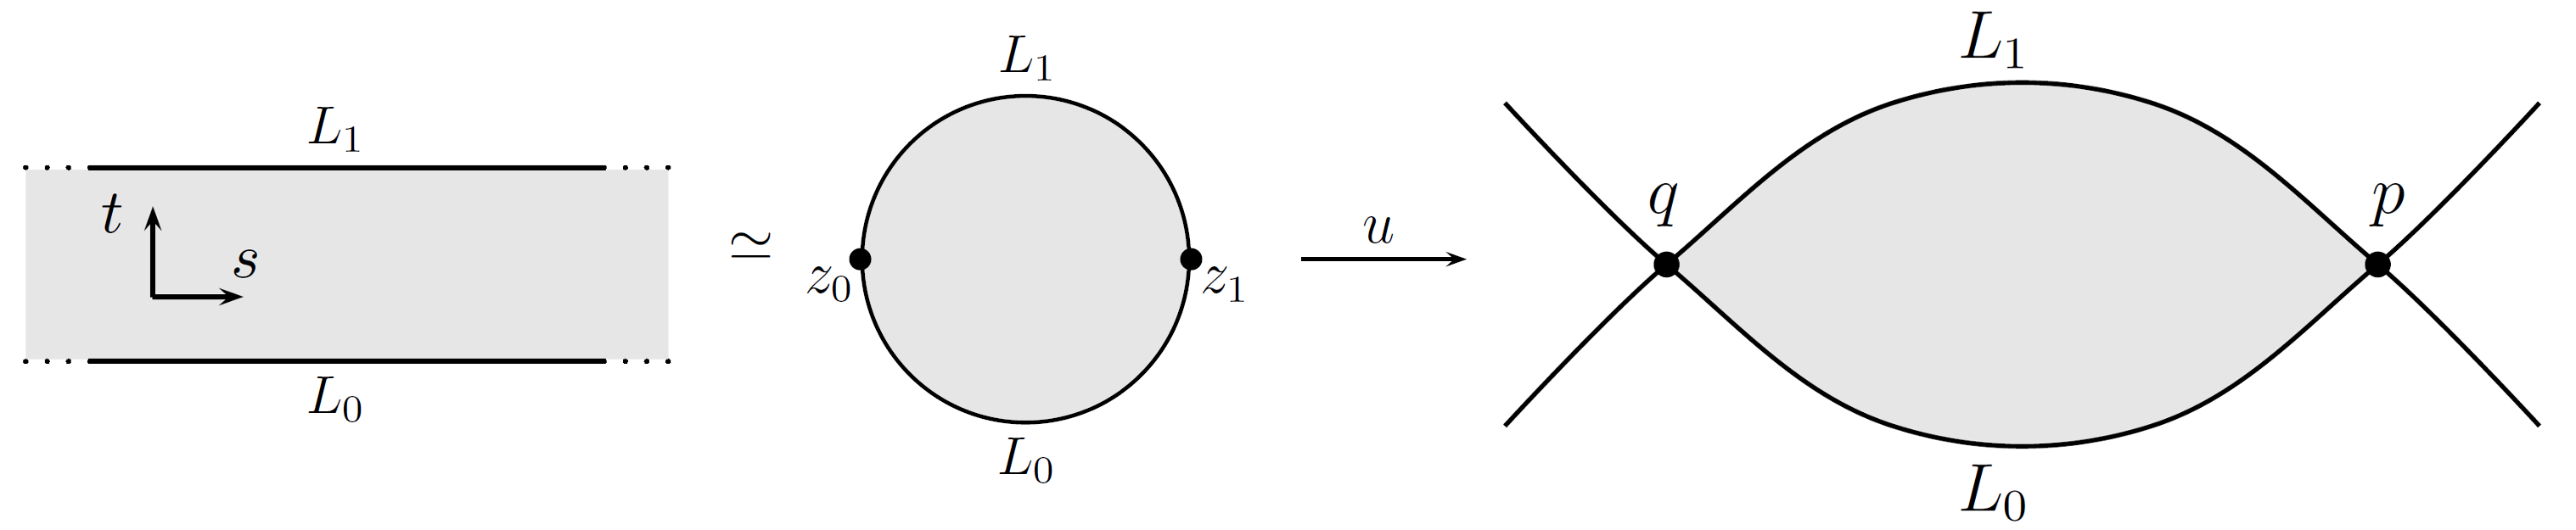
\includegraphics[width=0.9\linewidth]{fig02.png}
  \caption{属于 $\widehat{\mathcal M}(p,q;[u],J)$ 的一条 $J$-全纯条带 $u$。[来源：\cite{Aur13}]\hfill（原书 p.68）}
  \label{fig:02}
\end{figure}

\begin{Def}\label{def:5.12}
设 $M=(M,\omega,J)$ 是近复辛流形，$L_0,L_1\subset M$ 是紧致拉格朗日子流形，
且 $L_0\pitchfork L_1$。考虑 Cauchy--Riemann 问题 (57) 连同约束 (58) 与 (59)
的解 $u:\mathbb R\times[0,1]\to M$，它给出一个同伦类
$[u]\in\pi_2(M,L_0\cup L_1)
=\operatorname{Hom}_{\mathrm{hTop}}((B^2,S^1),(M,L_0\cup L_1))$，其中
$(B^2,S^1)\simeq(\mathbb D^2\setminus\{\pm1\},\mathbb R\times\{0\}\cup
\mathbb R\times\{1\})$ 与 $(M,L_0\cup L_1)$ 是带基点的拓扑空间对。

对固定的 $p,q\in\mathcal X(L_0,L_1)$，记
$\widehat{\mathcal M}(p,q;[u],J)$ 为表示 $[u]$ 的 (57)--(59) 之解构成的
\emph{模空间}，并令
$\mathcal M(p,q;[u],J):=\widehat{\mathcal M}(p,q;[u],J)/\mathbb R$。
\end{Def}

我们注意，$\mathbb R$ 通过沿 $s$ 坐标的平移自由作用在
$\widehat{\mathcal M}(p,q;[u],J)$ 上：若 $u(s,t)\in
\widehat{\mathcal M}(p,q;[u],J)$，则
$u_{\tilde s}(s,t):=u(s-\tilde s,t)\in\widehat{\mathcal M}(p,q;[u],J)$ 对所有
$\tilde s\in\mathbb R$ 成立。定义 $\mathcal M(p,q;[u],J)$ 时已把这一作用考虑在内。

现在有三方面问题妨碍我们为 $CF(L_0,L_1)$ 定义边界算子。也就是说，要使
$\widehat{\mathcal M}(p,q;[u],J)$ 成为“可驾驭”的空间，我们需要它具有如下性质：
\begin{itemize}
  \item \emph{横截性}，它保证 $\widehat{\mathcal M}(p,q;[u],J)$ 可被赋予有限维
  光滑流形的结构，其维数由 $[u]$ 的 Maslov 指标给出。
  \item \emph{紧致性}，只有在没有“能量堆积”使
  $\widehat{\mathcal M}(p,q;[u],J)$ 定义不良时才成立。
  \item \emph{可定向性}，它应与底拉格朗日子流形定向的选取相容。
\end{itemize}
然而，这些要求没有一项是先验满足的，因此需要额外假设。

先简要处理可定向性。下面的定义有意保持含糊，因为部分技术细节我们宁愿回避。
讲求实用的读者可以跳过。

\begin{Def}\label{def:5.13}
设 $L^n\subset M^{2n}$ 是拉格朗日子流形。假定 $L$ 可定向，即配有（一个等价类的）
处处非零 $n$-形式 $\theta_L\in\Omega^n(L)$，即一个体积形式。注意，由于光滑流形
特别是胞腔复形，可以考虑其骨架滤过。则称 $L$ 为：
\begin{itemize}
  \item \emph{自旋流形}，若可在 $1$-骨架 $L^{(1)}$ 上平凡化切丛 $TL$，且该平凡化
  可延拓到 $2$-骨架 $L^{(2)}$。这种平凡化的同伦类称为 $L$ 的\emph{自旋结构}；
  它存在当且仅当第二 Stiefel--Whitney 类
  $w_2(TL)\in H^2(L;\mathbb Z_2)$——$TL$ 的一个不变量——为零。
  \item 相对于某个固定 $\langle b\rangle\in H^2(M;\mathbb Z_2)$ 的
  \emph{相对自旋流形}，若 $w_2(TL)=\langle b\rangle|_L$。
\end{itemize}
\end{Def}

% [Tutor Note: 【含糊】定义 5.13 把自旋结构说成“$1$-骨架上可延拓到 $2$-骨架的
% 平凡化”，这只在胞腔复形上直观成立，严格定义须用 $TL$ 的 $2$-连通覆盖或
% $\operatorname{Spin}(n)$-主丛；相对自旋条件 $w_2(TL)=\langle b\rangle|_L$
% 则是为了在 $w_2(TM)\neq0$ 时仍能定向模空间。原文注明完整证明见
% \cite{Sei08} 第 12 章。]

假定 $L_0$ 与 $L_1$ 可定向且自旋，可以证明它们的自旋结构为
$\widehat{\mathcal M}(p,q;[u],J)$ 给出一个典范定向（\cite{Sei08} 第 12 章证明了
这一点）。不过，若 $\operatorname{char}(\mathbb K)=2$，这些假设都不必要。

\medskip
\noindent\fbox{\parbox{0.96\linewidth}{%
此后，我们总假定所有拉格朗日子流形都带有（隐含的）定向与自旋结构选取。}}
\medskip

\subsection{Maslov 指标}\label{sec:5.4}

同伦类 $[u]\in\pi_2(M,L_0\cup L_1)$（其中 $u$ 解 (57)--(59)）的 Maslov 指标
决定 $\widehat{\mathcal M}(p,q;[u],J)$ 的维数。实际情况其实更微妙（不熟悉此事的
读者可跳过下面这条注）：

\begin{Rem}\label{rem:5.14}
Cauchy--Riemann 问题 (57)--(59) 实际上是一个 \emph{Fredholm 问题}，即
$\bar\partial_J$ 在任一零点 $u$（即解）处的线性化 $D_{\bar\partial_J,u}$ 是
Fredholm 算子。可为 $[u]$ 指定其 \emph{Fredholm 指标}
$\operatorname{ind}([u]):=\dim(\ker(D_{\bar\partial_J,u}))
-\dim(\operatorname{coker}(D_{\bar\partial_J,u}))$，它实际上与下文将计算的
Maslov 指标一致。我们指出，哈密顿 Floer 理论实际上用另一个量来讨论，即
\emph{Conley--Zehnder 指标}。
\end{Rem}

回忆注 5.3 中拉格朗日 Grassmann 流形 $LGr(n)$ 的定义，它微分同胚于
$U(n)/O(n)$。可以证明，行列式映射 $\det:U(n)/O(n)\to S^1$ 的平方
$\det^2$ 诱导出同构 $\pi_1(LGr(n))\cong\pi_1(S^1)=\mathbb Z$。

\begin{Def}\label{def:5.15}
基于某个 $W\in LGr(n)$ 的环路 $\gamma:[0,1]\to LGr(n)$ 的\emph{Maslov 指标}
由 $\operatorname{im}(\det^2\circ\gamma)\subset S^1$ 的卷绕数
$\operatorname{ind}(\gamma):=w(\gamma,W)\in\mathbb Z$ 给出（这里把
$LGr(n)$ 等同于 $U(n)/O(n)$）。

另一方面，给定两条道路 $l_0,l_1:[0,1]\to LGr(n)$，满足
$l_0(0)\pitchfork l_1(0)$ 与 $l_0(1)\pitchfork l_1(1)$，定义
$l:=(l_0,l_1):t\in[0,1]\mapsto(l_0(t),l_1(t))\in LGr(n)\times LGr(n)$。
道路 $l_0,l_1$ 的\emph{Maslov 指标}是
\begin{equation}
\operatorname{ind}(l_0,l_1):=\left|\operatorname{im}(l)\cap
\overline{LGr(n)}\right|,
\label{eq:5.60}
\end{equation}
其中 $\overline{LGr(n)}:=\{(W,W')\in LGr(n)\times LGr(n)\mid
W\not\pitchfork W'\}$。换种说法，$\operatorname{ind}(l_0,l_1)$ 是
$l_0(t)$ 与 $l_1(t)$ 不横截的（带符号）次数，$0\le t\le1$ 递增。
\end{Def}

% [Tutor Note: 【易错】(60) 中横线并非闭包，而是“非横截对”之集：原文用
% $\overline{LGr(n)}$ 记 $\{(W,W')\mid W\not\pitchfork W'\}$，它是
% $LGr(n)\times LGr(n)$ 中余维 $1$ 的 Maslov 循环。$l$ 与该循环的相交数
% 带符号计数，符号由 $LGr(n)$ 的定向决定；这一符号约定经 (61)、(65) 一直
% 传到交点的次数 $\deg(p)$，故不能随意改动。]

让我们借助一个简单例子剖析指标对道路的几何意义。

\begin{Ex}\label{ex:5.16}
为简单起见，取 $l_0(t):=\mathbb R^n\subset\mathbb R^{2n}\cong\mathbb C^n$
为常值，并定义
$l_1(t):=(e^{i\varphi_1(t)}\mathbb R)\times\cdots\times
(e^{i\varphi_n(t)}\mathbb R)$，使所有角 $\varphi_k$ 一致地从 $-\pi/2$ 变到
$\pi/2$。$l_0$ 与 $l_1$ 的 Maslov 指标恰为
$\operatorname{ind}(l_0,l_1)=n$。这在 $n=1$ 时最易看出：此时 $l_0$ 是 $x$ 轴，
直线 $l_1(t)$ 逆时针地从 $l_1(0)=y$ 轴（其中 $\varphi_1(0)=-\pi/2$）转到
$l_1(1)=y$ 轴（其中 $\varphi_1(1)=\pi/2$），除 $\varphi(1/2)=0$ 时两条直线
实际重合外，其余时刻均与 $l_0$ 横截相交。\hfill$\blacklozenge$
\end{Ex}

现在考虑解 Cauchy--Riemann 问题 (57)--(59) 的 $J$-全纯条带
$u:\mathbb R\times[0,1]\to M$。对任意 $t\in[0,1]$，记
$q=u(-\infty,t)$ 与 $p=u(\infty,t)$。于是光滑映射 $u$ 给出辛拉回丛
$u^*TM=\{((s,t),(x,v))\in(\mathbb R\times[0,1])\times TM\mid u(s,t)=x\}$，
并可如下定义 $u$ 的 Maslov 指标。

\begin{Def}\label{def:5.17}
在为 $u^*TM\to\mathbb R\times[0,1]$ 选定平凡化之后（例如见 \cite{Mer14}
第 5 章），定义两条道路
$l_i(s):=((u|_{\mathbb R\times\{i\}})^*TL_i)|_{(-s,i)}
\cong T_{u(-s,i)}L_i$，其中 $s\in\overline{\mathbb R}=[-\infty,+\infty]$，
$i=0,1$；它们的像实际上落在 $LGr(n)$ 中（由注 5.3），并且每条 $l_i$ 都从
$T_pL_i$ 走向 $T_qL_i$，满足 $l_0(-\infty)\pitchfork l_1(-\infty)$ 与
$l_0(\infty)\pitchfork l_1(\infty)$（因为 $L_0\pitchfork L_1$）。

$J$-全纯条带 $u$ 的\emph{Maslov 指标}就是两条道路 $l_0,l_1$ 的 Maslov 指标，
$\operatorname{ind}([u]):=\operatorname{ind}(l_0,l_1)$，如定义 5.15 所述
（该定义对扩大的定义域 $\overline{\mathbb R}$ 仍然有效）。
\end{Def}

我们指出，$\operatorname{ind}(l_0,l_1)$ 实际上与 $u^*TM$ 所选取的平凡化无关，
且在 $\operatorname{Sp}(2n,\mathbb R)$ 中元素的共轭下不变。

% [Tutor Note: 【易错】定义 5.17 中 $l_i$ 的自变量是 $-s$，因此当 $s$ 从
% $-\infty$ 增至 $+\infty$ 时，$l_i$ 实际从 $T_pL_i$ 走向 $T_qL_i$。这一
% “反向参数化”是为与 (61) 中环路 $\gamma_u=\overline{l_0}*\lambda_p*l_1*
% \overline{\lambda_q}$ 的拼接次序配套；若漏掉负号，会得到
% $\operatorname{ind}([u])=\deg(p)-\deg(q)$ 而非推论 5.23 的结论。]

这使 $\operatorname{ind}([u])$ 良定义。此外，它在拼接下可加（进一步的性质以及
稍作修改的构造，见 \cite{Sei99} 第 4 节）。下面看它作为适当环路指标的等价表述。

\begin{Def}\label{def:5.18}
考虑 $\lambda_0,\lambda_1\in LGr(n)$，满足
$\lambda_0\pitchfork\lambda_1$。唯一确定变换
$A\in\operatorname{Sp}(2n,\mathbb R)$，使 $A(\lambda_0)=\mathbb R^n\subset
\mathbb C^n$ 且 $A(\lambda_1)=(i\mathbb R)^n\subset\mathbb C^n$。则称
$\lambda:t\in[0,1]\mapsto A^{-1}((e^{-i\pi t/2}\mathbb R)^n)\in LGr(n)$ 为从
$\lambda_0=\lambda(0)$ 到 $\lambda_1=\lambda(1)$ 的\emph{标准短路径}。
\end{Def}

\begin{Def}\label{def:5.19}
设 $u:\mathbb R\times[0,1]\to M$ 是解 Cauchy--Riemann 问题 (57)--(59) 的
$J$-全纯条带。按上一段定义道路 $l_0,l_1:\overline{\mathbb R}\to LGr(n)$，
并考虑如定义 5.18 的标准短路径
$\lambda_p,\lambda_q:[0,1]\to LGr(n)$，它们分别从 $T_pL_0$ 到 $T_pL_1$、
从 $T_qL_0$ 到 $T_qL_1$。

于是得到 $LGr(n)$ 中以 $T_qL_0$ 为基点的环路
$\gamma_u:=\overline{l_0}*\lambda_p*l_1*\overline{\lambda_q}$（横线表示逆道路）。
$u$ 的\emph{Maslov 指标}与相应的卷绕数一致：
\begin{equation}
\operatorname{ind}([u]):=\operatorname{ind}(\gamma_u)
=w(\gamma_u,T_qL_0)\,.
\label{eq:5.61}
\end{equation}
\end{Def}

\begin{Ex}\label{ex:5.20}
取 $M=\mathbb R^2$。则图 2 所示 $J$-全纯条带 $u$ 的 Maslov 指标可用如下技巧
计算：选取 $u^*TM$ 的平凡化，使道路 $l_0(s)=T_{u(-s,0)}L_0$ 等于常值切直线
$\mathbb R\times\{0\}$，并不失一般性地把 $L_1$ 参数化为向下的开口抛物线弧段
$\{(x,-x^2)\in\mathbb R^2\mid x\in[q,p]\}$（为清楚起见参看图 2）。

于是显然，道路 $l_1(s)=T_{u(-s,1)}L_1$ 只与 $l_0$ 不横截一次，即在 $s=0$ 处
（此处切线 $l_1(0)$ 平行于 $\mathbb R\times\{0\}$）。因此，按定义 5.19 用标准
短路径在 $T_qL_0$ 处闭合环路，便得 $\operatorname{ind}([u])=1$。
\hfill$\blacklozenge$
\end{Ex}

下面讨论如何为 Floer 复形配备 $\mathbb Z$-分次。这里，我们关于一阶 Chern 类
为 $2$-挠的假设开始发挥作用。

考虑纤维丛 $LGr(TM)\to M$，其纤维为
$LGr(TM)_x:=LGr(T_xM)\cong LGr(n)$（这是丛
$P\times_{\operatorname{Sp}(2n,\mathbb R)}LGr(n)$，其中 $P$ 是相伴的辛标架丛，
即 $M$ 上的主 $\operatorname{Sp}(2n,\mathbb R)$-丛），每个纤维都有万有覆盖
$\upsilon_x:\widetilde{LGr(T_xM)}\to LGr(T_xM)$。于是 $2c_1(TM)=0$ 让我们\footnote{遗憾的是，这又是一个超出本书范围的技术细节。它在
\cite{Fuk02b} 引理 2.6 或 \cite{Sei08} 第 (11j) 节中，在拉格朗日膜
（Lagrangian brane）的语境下得到处理。}可以把所有这些覆盖粘起来，形成覆盖空间
$\widetilde{LGr(TM)}\to LGr(TM)$，使得
$\widetilde{LGr(TM)}_x=\widetilde{LGr(T_xM)}$ 对所有 $x\in M$ 成立。
$\widetilde{LGr(TM)}$ 的元素称为 $TM$ 中的\emph{分次拉格朗日平面}。

现在，给定某条拉格朗日子流形 $L\subset M$ 上的截面
$s\in\Gamma(L,LGr(TM))$，$x\in L\mapsto T_xL\in LGr(T_xM)$，我们可能想问：
把 $s$ 提升为某个截面 $\tilde s\in\Gamma(L,\widetilde{LGr(TM)})$ 的障碍是什么？
也就是说，如何得到交换图
\begin{equation}
\begin{tikzcd}
& \widetilde{T_xL}\in\widetilde{LGr(T_xM)} \arrow[d,"\upsilon_x"] \\
x\in L \arrow[ur,"\tilde s"] \arrow[r,"s"'] & T_xL\in LGr(T_xM)
\end{tikzcd}
\label{eq:5.62}
\end{equation}
事实证明，我们需要 $L$ 的 Maslov 类消没：

\begin{Def}\label{def:5.21}
设 $(M,\omega)$ 是满足 $2c_1(TM)=0$ 的辛流形，于是可为每个
$W\in LGr(T_xM)$ 指定一个“相位” $\phi(W)\in S^1$，并选取提升
$\tilde\phi(W)\in\mathbb R$ 满足 $\phi(W)=e^{2\pi i\tilde\phi(W)}$。则对拉格朗日
子流形 $L\subset M$，可定义其“相位函数” $\phi_L:L\to S^1$，
$\phi_L(x):=\phi(T_xL)$。$L$ 的\emph{Maslov 类}恰为\footnote{注意，$\mathbb Z$
可除，故 $\operatorname{Ext}(H_0(L),\mathbb Z)$ 消没，从而
$H^1(L;\mathbb Z)\cong\operatorname{Hom}(H_1(L),\mathbb Z)$。又，在 $L$ 的连通
分支上，Hurewicz 定理告诉我们
$H_1(L)\cong\pi_1(L)^{\mathrm{ab}}=\pi_1(L)/[\pi_1(L),\pi_1(L)]$，而 $\mathbb Z$
交换保证 $\operatorname{Hom}(\pi_1(L),\mathbb Z)\cong
\operatorname{Hom}(\pi_1(L)^{\mathrm{ab}},\mathbb Z)$。}
\begin{equation}
\mu_L\equiv[\phi_L]:=\pi_1(\phi_L)\in\operatorname{Hom}(\pi_1(L),\pi_1(S^1))
\cong H^1(L;\mathbb Z)\,.
\label{eq:5.63}
\end{equation}
此外，选取映射 $\tilde\phi_L:L\to\mathbb R$ 提升 $\phi_L$，即使其落入交换图
\begin{equation}
\begin{tikzcd}
& \tilde\phi(T_xL)\in\mathbb R \arrow[d,"\exp(2\pi i\,\cdot\,)"] \\
x\in L \arrow[ur,"\tilde\phi_L"] \arrow[r,"\phi_L"'] & \phi(T_xL)\in S^1
\end{tikzcd}
\label{eq:5.64}
\end{equation}
便得到带有分次提升 $\tilde\phi_L$ 的\emph{分次拉格朗日子流形}
$(L,\tilde\phi_L)$。
\end{Def}

% [Tutor Note: 【含糊】原文说“可为每个 $W$ 指定相位 $\phi(W)\in S^1$”，其
% 依据是 $\det^2:U(n)/O(n)\to S^1$ 的万有覆盖；$2c_1(TM)=0$ 保证这些局部
% 相位能沿 $M$ 整体粘接。相位函数的提升 $\tilde\phi_L$ 一旦选定，交点的次数
% $\deg(p)$ 便确定；把 $\tilde\phi_L$ 整体平移整数 $k$，所有次数同时平移
% $k$，Floer 复形只作整体平移，上同调不变。]

现在选取横截相交的分次拉格朗日子流形
$(L_0,\tilde\phi_{L_0}),(L_1,\tilde\phi_{L_1})\subset M$，满足
$[\phi_{L_0}]=[\phi_{L_1}]=0$，于是存在如图 (62) 的截面。取任意
$p\in L_0\cap L_1$。则存在一条受偏爱的（同伦类的）道路
$l_p:[0,1]\to LGr(T_pM)$，使 $l_p(0)=T_pL_0$ 且 $l_p(1)=T_pL_1$，即覆盖映射
$\upsilon_p$ 在观察万有覆盖 $\widetilde{LGr(T_pM)}$ 后所选出的那一条。

\begin{Def}\label{def:5.22}
设 $(L_0,\tilde\phi_{L_0}),(L_1,\tilde\phi_{L_1})\subset M$ 是 Maslov 类消没的
分次拉格朗日子流形，$p\in L_0\cap L_1$。设 $l_p:[0,1]\to LGr(T_pM)$ 是上一段
所述道路，$\lambda_p:[0,1]\to LGr(T_pM)$ 是从 $T_pL_0$ 到 $T_pL_1$ 的标准短
路径。则 $p$ 的\emph{次数}由
\begin{equation}
\deg(p):=w(\gamma_p)
\label{eq:5.65}
\end{equation}
给出，其中 $\gamma_p:=l_p*\overline{\lambda_p}$ 是以 $T_pL_0$ 为基点的环路。
\end{Def}

在适当地等同切空间 $T_x(L_0\cap L_1)$ 之后，定义 5.19 与 5.22 的直接推论是：

\begin{Cor}\label{cor:5.23}
设 $u:\mathbb R\times[0,1]\to M$ 是解 Cauchy--Riemann 问题 (57)--(59) 的
$J$-全纯条带，其中 $L_0$ 与 $L_1$ 是横截相交、Maslov 类消没
（$[\phi_{L_0}]=[\phi_{L_1}]=0$）的分次拉格朗日子流形。则
\[
\operatorname{ind}([u])=\deg(q)-\deg(p).
\]
特别地，$\operatorname{ind}([u])$ 只依赖于由 $u$ 相连的两个生成元 $p,q$，
因此可为 $CF(L_0,L_1)$ 配备 $\mathbb Z$-分次：
\[
CF^n(L_0,L_1):=\bigoplus_{\substack{p\in\mathcal X(L_0,L_1):\\
\deg(p)=n}}\Lambda_{\mathbb K}\cdot p\,,
\qquad n\in\mathbb Z.
\]
\end{Cor}

% [Tutor Note: 【易错】推论 5.23 的符号取决于 (61) 的环路次序与 (58) 的端点
% 约定：$q$ 是负端（$s\to-\infty$）、$p$ 是正端（$s\to+\infty$），故
% $\operatorname{ind}=\deg(q)-\deg(p)$。若把 $u$ 反向参数化，得到的是
% $\deg(p)-\deg(q)$，这正是 (74) 中 $\partial$ 提升次数 $+1$ 的来源：
% 从 $p$ 到 $q$ 的条带使 $\deg(q)=\deg(p)+1$。]

若没有假设 $2c_1(TM)=0$ 与 $[\phi_{L_0}]=[\phi_{L_1}]=0$，我们仅得到
$\mathbb Z_2$-分次（这一替代方案在 \cite{Sei99} 第 4 节中简要讨论）。

\medskip
\noindent\fbox{\parbox{0.96\linewidth}{%
此后，我们假定所有（可定向自旋的）拉格朗日子流形都是分次的，且 Maslov 类消没。}}
\medskip

\subsection{横截性}\label{sec:5.5}

模空间 $\widehat{\mathcal M}(p,q;[u],J)$ 的横截性处理起来更具挑战性，尤其在
底层理论方面。

\begin{Rem}\label{rem:5.24}
沿用注 5.14 的技术要点：若线性化 $D_{\bar\partial_J,u}$ 的所有零点都是正则的，
即 $D_{\bar\partial_J,u}$ 对所有 $u\in\widehat{\mathcal M}(p,q;[u],J)$ 都满射，
则横截性得以实现。
\end{Rem}

$L_0\pitchfork L_1$ 情形的解决办法，是允许 $\omega$-相容近复结构依赖 $t$，
即把 (57) 中的 $J$ 换成 $J_t$，$t\in[0,1]$（形式上，取
$J\in C^\infty([0,1],\mathcal J(M,\omega))$ 并写 $J_t:=J(t,\,\cdot\,)$）。

当我们试图在最一般情形 $L_0\not\pitchfork L_1$ 下定义 $CF(L_0,L_1)$ 时，也会
遇到同样的策略——若想在 $CF(L_i,L_i)$ 中找到恒等态射，这种情形确实必须研究！
事实上，为摆脱拉格朗日子流形的横截性要求，我们考虑时间依赖的哈密顿函数
$H\in C^\infty([0,1]\times M)$，使得
$L_0\pitchfork(\phi_H^1)^{-1}(L_1)$，其中 $\phi_H^1:M\to M$ 是相应
$t$-依赖哈密顿向量场 $X_H\in\mathfrak X([0,1]\times M)$ 的哈密顿微分同胚。
于是方程 (57) 变成微扰 PDE，微扰由 $X_H$ 给出：
\begin{equation}
\bar\partial_{J,H}(u):=\partial_su+J_t(u)(\partial_tu-X_{H_t}(u))=0\,.
\label{eq:5.66}
\end{equation}
（这有时称为 \emph{Floer 方程}，$\bar\partial_{J,H}$ 称为 Floer 微分。）边界条件
必须相应修改。有限能量约束 (59) 成为：
\begin{equation}
E(u)=\frac12\int_{-\infty}^{+\infty}\!\!\int_0^1
\left(|\partial_su|^2+|\partial_tu-X_{H_t}(u)|^2\right)ds\,dt<\infty,
\label{eq:5.67}
\end{equation}
并且我们仍要求 $u(s,i)\in L_i$（$i=0,1$）。然而，$s\to\pm\infty$ 时的渐近线
因下面的观察而改变。

\begin{Rem}\label{rem:5.25}
微扰 Cauchy--Riemann 方程 (66) 可按如下方式化为 (57) 形式的齐次
Cauchy--Riemann 方程。设 $\phi_H^t:M\to M$ 是 $X_H$ 的流，并考虑 $u$ 在该流下
的原像 $\tilde u:\mathbb R\times[0,1]\to M$，
$\tilde u(s,t):=(\phi_H^t)^{-1}(u(s,t))$，于是链式法则给出
$\partial_t\tilde u=(\phi_H^t)^{-1}_*(\partial_tu-X_H)$。再定义
$\tilde J_t:=(\phi_H^t)^{-1}_*(J_t)$。则 (66) 呈现熟悉的面貌
\[
\partial_s\tilde u+\tilde J_t(\tilde u)\partial_t\tilde u=0,
\]
这是我们有把握其解为 $\tilde J$-全纯条带 $\tilde u$ 的 PDE，且
$\tilde u(s,0)=u(s,0)\in L_0$，
$\tilde u(s,1)=(\phi_H^1)^{-1}(u(s,1))\in(\phi_H^1)^{-1}(L_1)$。
\end{Rem}

% [Tutor Note: 【含糊】注 5.25 中“$\tilde J_t:=(\phi_H^t)^{-1}_*(J_t)$”是把
% 近复结构沿微分同胚拉回；要验证 $\tilde J_t$ 仍与某个辛形式相容，须同时
% 拉回 $\omega$ 或检查 $\tilde J_t^2=-\mathrm{id}$ 与相容性。原文未说明
% $(\phi_H^t)^{-1}_*$ 作用在 $(1,1)$-张量上，也未验证该拉回保持 $\tilde J$
% 的可积性以外的性质；这里照印，细节见 \cite{Mer14} 第 3 章。]

由上一注，Floer 复形的定义 5.11 现在需要修改
$\mathcal X(L_0,L_1)\equiv\mathcal X(L_0,L_1;H):=L_0\cap(\phi_H^1)^{-1}(L_1)$，
由于 $L_0\pitchfork(\phi_H^1)^{-1}(L_1)$，它仍是离散有限集。生成元是按流线
$\gamma:[0,1]\to M$（按定义满足 $\dot\gamma(t)=X_{H_t}(t,\gamma(t))$）微扰的
交点，使得 $\gamma(0)\in L_0$ 且 $\gamma(1)\in L_1$。相应地，Floer 微分计数
形如 $\mathcal M(p,q;[u],J,H)$ 的模空间中的\emph{微扰} $J$-全纯条带，这些模空间
现在也依赖于 $H$。

\begin{Rem}\label{rem:5.26}
（警告）在选取合适的 $H\in C^\infty([0,1]\times M)$ 使
$L_0\pitchfork(\phi_H^1)^{-1}(L_1)$ 时，我们忽略了一个非平凡事实：$H$ 实际上应
取自 $\mathcal H_{\mathrm{reg}}\subset C^\infty([0,1]\times M)$，即所有这样的
哈密顿函数之子集：其哈密顿微分同胚对某对拉格朗日子流形满足上述横截性。不过，
这并不使我们的分析失效，因为 $\mathcal H_{\mathrm{reg}}$ 原来是
$C^\infty([0,1]\times M)$ 的稠密子集（更精确地说，是 Baire 意义下的第二纲集；
参看 \cite{Sal97} 定理 1.24）。

类似地，保证线性化 $D_{\bar\partial_J,u}$ 满射（见注 5.24）的时间依赖近复结构
$J$，实际上也应属于稠密子集
$\mathcal J_{\mathrm{reg}}\subset C^\infty([0,1],\mathcal J(M,\omega))$。

选取数据 $(J,H)$ 时，我们把这些考虑放在心上。
\end{Rem}

% [Tutor Note: 【背景】$\mathcal H_{\mathrm{reg}}$ 稠密但不一定开；Floer 理论
% 的“通有选取”通常指存在稠密 $G_\delta$ 集使所有条带正则。原文用“Baire 第二
% 纲”表述，只保证稠密性，未保证稳定性；实际使用中还需横截性论证对每个
% 同伦类分别成立。]

让我们从略有不同的视角考察微扰问题 (66)，即 \cite{Oh91}、\cite{McS94} 与
\cite{Mer14} 第 3 章所提供的视角。

\begin{Def}\label{def:5.27}
设 $(M,\omega)$ 是辛流形，$L_0,L_1\subset M$ 是任意拉格朗日子流形，
$H\in C^\infty([0,1]\times M)$ 是时间依赖哈密顿量。定义\emph{道路空间}
\[
\mathcal P=\mathcal P(L_0,L_1):=\{\gamma\in C^\infty([0,1],M)\mid
\gamma(0)\in L_0,\ \gamma(1)\in L_1\}.
\]
这是具有可数多个连通分支的无穷维光滑流形，其切空间为
\[
T_\gamma\mathcal P=\Gamma(\gamma^*TM)\cong\Gamma_\gamma(TM)
:=\{\xi\in C^\infty([0,1],TM)\mid\xi(t)\in T_{\gamma(t)}M\},
\]
对每个 $\gamma\in\mathcal P$。我们通过它所等同的 $C^\infty(\mathcal P)$-线性映射
$\mathfrak X(\mathcal P)\to C^\infty(\mathcal P)$ 定义闭 $1$-形式
$a_H\in\Omega^1(\mathcal P)$：
\begin{equation}
\begin{aligned}
(a_H)_\gamma(\xi)
&:=\int_0^1\left(\omega_{\gamma(t)}(\xi(t),\dot\gamma(t))
-(dH_t)_{\gamma(t)}(\xi(t))\right)dt\\
&=\int_0^1\omega_{\gamma(t)}
\left(\xi(t),\dot\gamma(t)-X_{H_t}(\gamma(t))\right)dt,
\end{aligned}
\label{eq:5.68}
\end{equation}
其中 $\gamma\in\mathcal P$（于是
$\dot\gamma:=\frac{d}{dt}\big|_t\gamma\in\Gamma_\gamma(TM)$），
$\xi\in T_\gamma\mathcal P$；最后一个等式利用了
$dH_t=\omega(\,\cdot\,,X_{H_t}):\mathfrak X(M)\to C^\infty(M)$，即哈密顿向量场
的定义（见定义 5.4）。注意 $a_H$ 的闭性是 $\omega$ 闭性的直接推论。
\end{Def}

于是不难看出：

\begin{Cor}\label{cor:5.28}
设 $(M,\omega)$ 是辛流形，$L_0,L_1\subset M$ 是任意拉格朗日子流形，
$H\in C^\infty([0,1]\times M)$ 是生成流 $\phi_H^t:M\to M$ 的时间依赖哈密顿
函数。如上定义 $a_H\in\Omega^1(\mathcal P)$。则 $\gamma\in\mathcal P$ 是 $a_H$
的零点，$\gamma\in\operatorname{zeros}(a_H)$，当且仅当 $\gamma$ 是流线，即
$\gamma(t)=\phi_H^t(x)$ 对某个 $x\in L_0$ 成立。特别地，由时间 $0$ 处的求值给出
一个双射：
\begin{equation}
\{\gamma\in\operatorname{zeros}(a_H)\}\longleftrightarrow
\{\gamma(0)=x\in L_0\cap(\phi_H^1)^{-1}(L_1)\}\,.
\label{eq:5.69}
\end{equation}
\end{Cor}

推论 5.28 告诉我们，可以把 Floer 复形 $CF(L_0,L_1)$ 的生成元等同于闭
$1$-形式 $a_H$ 的零点；我们称后者为从 $L_0$ 到 $L_1$ 的\emph{时间 $1$ 哈密顿弦}。

不过，我们还能改进这一解释。

\begin{Def}\label{def:5.29}
设 $(M,\omega)$ 是辛流形，$L_0,L_1\subset M$ 是任意拉格朗日子流形。如上定义
道路空间 $\mathcal P=\mathcal P(L_0,L_1)$，并为
$\mathcal P=\bigsqcup_{k\in I}\mathcal P_k$ 的每个连通分支选取固定的参考道路
$\gamma_k\in\mathcal P_k$。对 $\gamma\in\mathcal P_k$，称\footnote{这一术语并非标准。}
$\bar\gamma\in C^\infty(\overline{\mathbb R}\times[0,1],M)$ 为
$\gamma$ 的\emph{桥}，若 $\bar\gamma(-\infty,\,\cdot\,)=\gamma_k$，
$\bar\gamma(+\infty,\,\cdot\,)=\gamma$，且
$\bar\gamma(s,\,\cdot\,)\in\mathcal P_k$ 对所有
$s\in\overline{\mathbb R}$ 成立（于是也可写
$\bar\gamma\in C^\infty(\overline{\mathbb R},\mathcal P_k)$）。
\end{Def}

\begin{Def}\label{def:5.30}
设 $(M,\omega)$ 是辛流形，$L_0,L_1\subset M$ 是拉格朗日子流形，
$H\in C^\infty([0,1]\times M)$。设 $\mathcal P=\mathcal P(L_0,L_1)$ 是相应的
道路空间，并固定某个 $\gamma_0\in\mathcal P$，使
$\gamma_0(0)=q\in L_0\cap(\phi_H^1)^{-1}(L_1)$ 是 Floer 复形
$CF(L_0,L_1)$ 的微扰生成元（或等价地由 (69)，使
$\gamma_0\in\operatorname{zeros}(a_H)$）。定义\emph{哈密顿作用量泛函}
$A_H:\mathcal P\to\mathbb R$ 为
\begin{equation}
A_H(\gamma):=\int_{\mathbb R\times[0,1]}\bar\gamma^*\omega
-\int_0^1H_t(\gamma(t))dt,
\label{eq:5.70}
\end{equation}
其中 $\bar\gamma\in C^\infty(\mathbb R\times[0,1],M)$ 是 $\gamma\in\mathcal P$ 的
任一桥，满足 $\bar\gamma(-\infty)=\gamma_0$（为使其有意义，注意 $\gamma$ 必须与
$\gamma_0$ 属于 $\mathcal P$ 的同一连通分支！）。
\end{Def}

就目前所写，$A_H$ 的定义仍不完整，因为我们必须证明它与桥 $\bar\gamma$ 的具体
选取无关——事实上我们小小地作弊了：若不对 $M,L_0,L_1$ 作适当假设，在
$\mathcal P=\mathcal P(L_0,L_1)$ 上定义哈密顿作用量泛函一般是不可能的，人们被迫
改在其 \emph{Novikov 覆盖} $\overline{\mathcal P}$ 上工作。这是由所有对
$[\gamma,\bar\gamma]$ 构成的空间，其中 $\bar\gamma$ 是 $\gamma\in\mathcal P$ 的
桥；在把相对于 $\partial(\mathbb R\times[0,1])$ 同伦的所有桥等同之后得到。再多做
一些工作，可以进一步改造 $\overline{\mathcal P}$，得到覆盖映射
$\pi:\overline{\mathcal P}\to\mathcal P$，在 $H=0$ 时满足
$dA_H=\pi^*(a_H)$（例如见 \cite{Oh91} 命题 13.5.1）。这在微扰情形 $H\neq0$ 下
仍然成立：

\begin{Lem}\label{lem:5.31}
设 $A_H:\overline{\mathcal P}\to\mathbb R$ 是哈密顿作用量泛函 (70)，
$a_H\in\Omega^1(\mathcal P)$ 是 $1$-形式 (68)。则
$dA_H=\pi^*(a_H)$。因此 $A_H$ 的临界点与 $a_H$ 的零点一致，
$\operatorname{crit}(A_H)=\operatorname{zeros}(a_H)$。
\end{Lem}

% [Tutor Note: 【易错】作用量泛函只在 Novikov 覆盖 $\overline{\mathcal P}$ 上
% 良定义，其理由与 (70) 中桥的选取有关：不同桥相差闭曲面，$\int\bar\gamma^*\omega$
% 的改变量是辛面积，一般非零。因此 $dA_H=\pi^*(a_H)$ 中的 $\pi^*$ 不可省；
% 原文在 $H=0$ 处说明，并称微扰情形同理。证明依赖 $\omega$ 闭与 Stokes 定理。]

这与推论 5.28 一起，帮助我们细化对一般 Floer 复形
$CF(L_0,L_1;H)$ 生成元的解释：
\begin{equation}
\{\gamma(0)=x\in\mathcal X(L_0,L_1;H)\}\longleftrightarrow
\{\gamma\in\operatorname{crit}(A_H)\}\,.
\label{eq:5.71}
\end{equation}

引理 5.31 还引出下面两个定义。

\begin{Def}\label{def:5.32}
设 $(M,\omega,J)$ 是近复辛流形，$J\in\mathcal J(M,\omega)$，
$L_0,L_1\subset M$ 是拉格朗日子流形，$H\in C^\infty([0,1]\times M)$。定义
$L^2$-内积
\[
\langle\!\langle\xi,\zeta\rangle\!\rangle_J
:=\int_0^1(g_J)_{\gamma(t)}(\xi(t),\zeta(t))dt
=\int_0^1\omega_{\gamma(t)}(J_{\gamma(t)}(\xi(t)),\zeta(t))dt,
\]
其中 $\gamma\in\mathcal P$，$\xi,\zeta\in T_\gamma\mathcal P$。然后记
$\nabla_JA_H\in\mathfrak X(\mathcal P)$ 为向量场
\begin{equation}
\nabla_JA_H(\gamma):=J(\gamma)(\dot\gamma-X_H(\,\cdot\,,\gamma))\in
T_\gamma\mathcal P
\label{eq:5.72}
\end{equation}
（其中 $J(\gamma)\equiv J_{\gamma(\,\cdot\,)}$）。显式地，对任意 $t\in[0,1]$ 有
$\nabla_JA_H(\gamma)(t):=J_{\gamma(t)}(\dot\gamma(t)-X_{H_t}(\gamma(t)))
\in T_{\gamma(t)}M$。
\end{Def}

\begin{Lem}\label{lem:5.33}
向量场 $\nabla_JA_H\in\mathfrak X(\mathcal P)$ 是 $A_H$ 关于
$\langle\!\langle\,\cdot\,,\,\cdot\,\rangle\!\rangle_J$ 的 $L^2$-梯度，即
$(dA_H)_\gamma(\xi)=\langle\!\langle\nabla_JA_H(\gamma),\xi\rangle\!\rangle_J$
对所有 $\gamma\in\mathcal P$ 与 $\xi\in T_\gamma\mathcal P$ 成立。
\end{Lem}

\begin{proof}
这是直接计算。取任意 $\gamma\in\mathcal P$ 与 $\xi\in T_\gamma\mathcal P$，则
\begin{align*}
(dA_H)_\gamma(\xi)
&=\int_0^1\omega_{\gamma(t)}\left(\xi(t),\dot\gamma(t)
-X_{H_t}(\gamma(t))\right)dt\\
&=\int_0^1\omega_{\gamma(t)}\left(J^2_{\gamma(t)}
\left(\dot\gamma(t)-X_{H_t}(\gamma(t))\right),\xi(t)\right)dt\\
&=\int_0^1(g_J)_{\gamma(t)}\left(J_{\gamma(t)}
\left(\dot\gamma(t)-X_{H_t}(\gamma(t))\right),\xi(t)\right)dt\\
&=\int_0^1(g_J)_{\gamma(t)}\left(\nabla_JA_H(\gamma)(t),\xi(t)\right)dt
=\langle\!\langle\nabla_JA_H(\gamma),\xi\rangle\!\rangle_J.
\end{align*}
\end{proof}

% [Tutor Note: 【易错】证明第二行用了 $J^2=-\mathrm{id}$ 与 $\omega$ 的反对称性：
% $\omega(J^2v,\xi)=\omega(-v,\xi)=\omega(\xi,v)$，故与第一行同值；第三行再用
% $g_J=\omega(J\,\cdot\,,\,\cdot\,)$。若采用文献中相反的 $g_J$ 约定，此处
% $\nabla_JA_H$ 与 (73) 的流方向都会整体变号。]

用刚刚建立的语言，微扰 Cauchy--Riemann 方程 (66) 可以写成
\begin{equation}
\frac{d}{ds}u(s)+\nabla_JA_H(u(s))=0,
\label{eq:5.73}
\end{equation}
这是 $\mathcal P$ 上的一个 ODE；其中我们把 $J$-全纯条带
$u:\mathbb R\times[0,1]\to M$ 重新解释为映射 $u:\mathbb R\to\mathcal P$，即
$A_H$ 的（有界）负梯度流线。解 $u\in\mathcal M(p,q;[u],J,H)$ 的能量可通过
作用量泛函表示为
\[
E(u)=A_H(\gamma_-)-A_H(\gamma_+),
\]
其中 $\gamma_\pm\in\operatorname{crit}(A_H)$ 满足 $\gamma_-(0)=q$ 与
$\gamma_+(0)=p$。显然这说得通：$\mathcal M(p,q;[u],J,H)$ 非空，当且仅当
$A_H(\gamma_-)>A_H(\gamma_+)$ 或 $\gamma_-=\gamma_+$。

然而，这一替代立场并未给我们带来更多好处，我们宁愿把焦点保持在\footnote{确实，这正是 Andreas Floer 在发展 Floer 同调时的天才直觉：把提法不当的 ODE (73) 看作 PDE (57) 的微扰，而 (57) 的解正是众所周知的 $J$-全纯条带。}$M$ 上的微扰
PDE (66)。对底层 Floer 理论机制感兴趣的读者，再次被引向 \cite{Oh91}。

\medskip
\noindent\fbox{\parbox{0.96\linewidth}{%
此后，我们隐含地选取时间依赖近复结构
$J\in C^\infty([0,1],\mathcal J(M,\omega))$ 与哈密顿量
$H\in C^\infty([0,1]\times M)$，把分析转向未必横截相交的拉格朗日子流形的
微扰 Cauchy--Riemann 问题 (66)。}}
\medskip

\subsection{紧致性}\label{sec:5.6}

在着手定义 Floer 微分之前，必须先处理光滑流形
$\widehat{\mathcal M}(p,q;[u],J,H)$ 的紧致性问题。由于下面这个结果（例如见
\cite{Sal97} 命题 3.3），它或许是第 5.3 节所列三项要求中最微妙的一项。

\begin{Pro}[Gromov 紧致性定理]\label{prop:5.34}
考虑一列 $J$-全纯条带
$(u_n)_{n\in\mathbb N}\subset\widehat{\mathcal M}(p,q;[u],J,H)$，其能量一致有界，
$\sup_{n\in\mathbb N}E(u_n)<\infty$。则存在有限多个点
$(s_j,t_j)\equiv s_j+it_j=:z_j\in\mathbb D^2\setminus\{\pm1\}$（例如
$j=1,\dots,l$），以及一个子列
$(u_{n_k})_{k\in\mathbb N}\subset\widehat{\mathcal M}(p,q;[u],J,H)$，它一致收敛
到 (66) 的某个解 $u\in\widehat{\mathcal M}(p,q;[u],J,H)$，且其导数在
$(\mathbb D^2\setminus\{\pm1\})\setminus\{z_1,\dots,z_l\}$ 的紧子集上收敛。
\end{Pro}

% [Tutor Note: 【含糊】Gromov 紧致性定理只说“在冒泡点之外 $C^\infty$ 收敛”，
% 既未说明极限对象是稳定映射（可能带气泡树），也未说明气泡的能量；证明需要
% 先验 $C^0$ 界、椭圆正则性与单调性，超出本书范围。原文把它当作黑箱使用，
% 并在 (75) 的粘接定理中反向补回。]

\begin{Def}\label{def:5.35}
考虑上一命题中 $J$-全纯曲线之子列
$(u_{n_k})_{k\in\mathbb N}\subset\widehat{\mathcal M}(p,q;[u],J,H)$。则导数
$(du_{n_k})_k$ 在那些 $z_j=(s_j,t_j)\in\mathbb R\times[0,1]$ 处无界，这造成
$k\to\infty$ 时的“能量集中”。我们说极限条带 $u$ 出现一个\emph{冒泡}。这种
“冒泡”现象有三种可能（见图 3）：
\begin{itemize}
  \item \emph{条带断裂}，发生在
  $\lim_{k\to\infty}|(du_{n_k})(z)|=\infty$ 于 $z=(s,t)\in\mathbb R\times[0,1]$
  且 $s\to\pm\infty$ 时，于是极限条带“断裂”（即具有一个中间节点）。若把每个
  分量看作 $J$-全纯圆盘，这等价于在端点 $p,q$ 之一处出现气泡。形式上，存在
  序列 $a_n\to\pm\infty$，使平移后的条带 $u_n(\,\cdot\,-a_n,\,\cdot\,)$ 收敛到
  一个非常值极限条带。
  \item \emph{圆盘冒泡}，发生在
  $\lim_{k\to\infty}|(du_{n_k})(z)|=\infty$ 于某个 $z=(s,t)\in\mathbb R\times
  [0,1]$、$t\in\{0,1\}$ 时，于是极限条带具有一个气泡，它由一张 $J$-全纯圆盘
  构成，其边界与 $L_0$ 或 $L_1$ 相交——并且在适当重标度后完全含于 $L_0$ 或
  $L_1$ 中。
  \item \emph{球面冒泡}，发生在
  $\lim_{k\to\infty}|(du_{n_k})(z)|=\infty$ 于某个
  $z=(s,t)\in(\mathbb R\times[0,1])^\circ$ 时，于是极限条带出现一个气泡，
  它在适当重标度后是一张 $J$-全纯球面 $\mathbb C P^1\to M$，并在
  $\operatorname{im}(u)$ 的某个内点处与其横截相交。
\end{itemize}
\end{Def}

条带断裂正是 Floer 微分在没有圆盘冒泡与球面冒泡时平方为零的原因。后两者不可取，
因为它们还妨碍 $\widehat{\mathcal M}(p,q;[u],J,H)$ 的横截性；第 5.5 节所采用的
微扰 $J\in C^\infty([0,1],\mathcal J(M,\omega))$ 与
$H\in C^\infty([0,1]\times M)$ 这次也解决不了问题！因此，我们希望保留条带断裂
现象，而舍弃圆盘冒泡与球面冒泡。\begin{figure}[htbp]
  \centering
  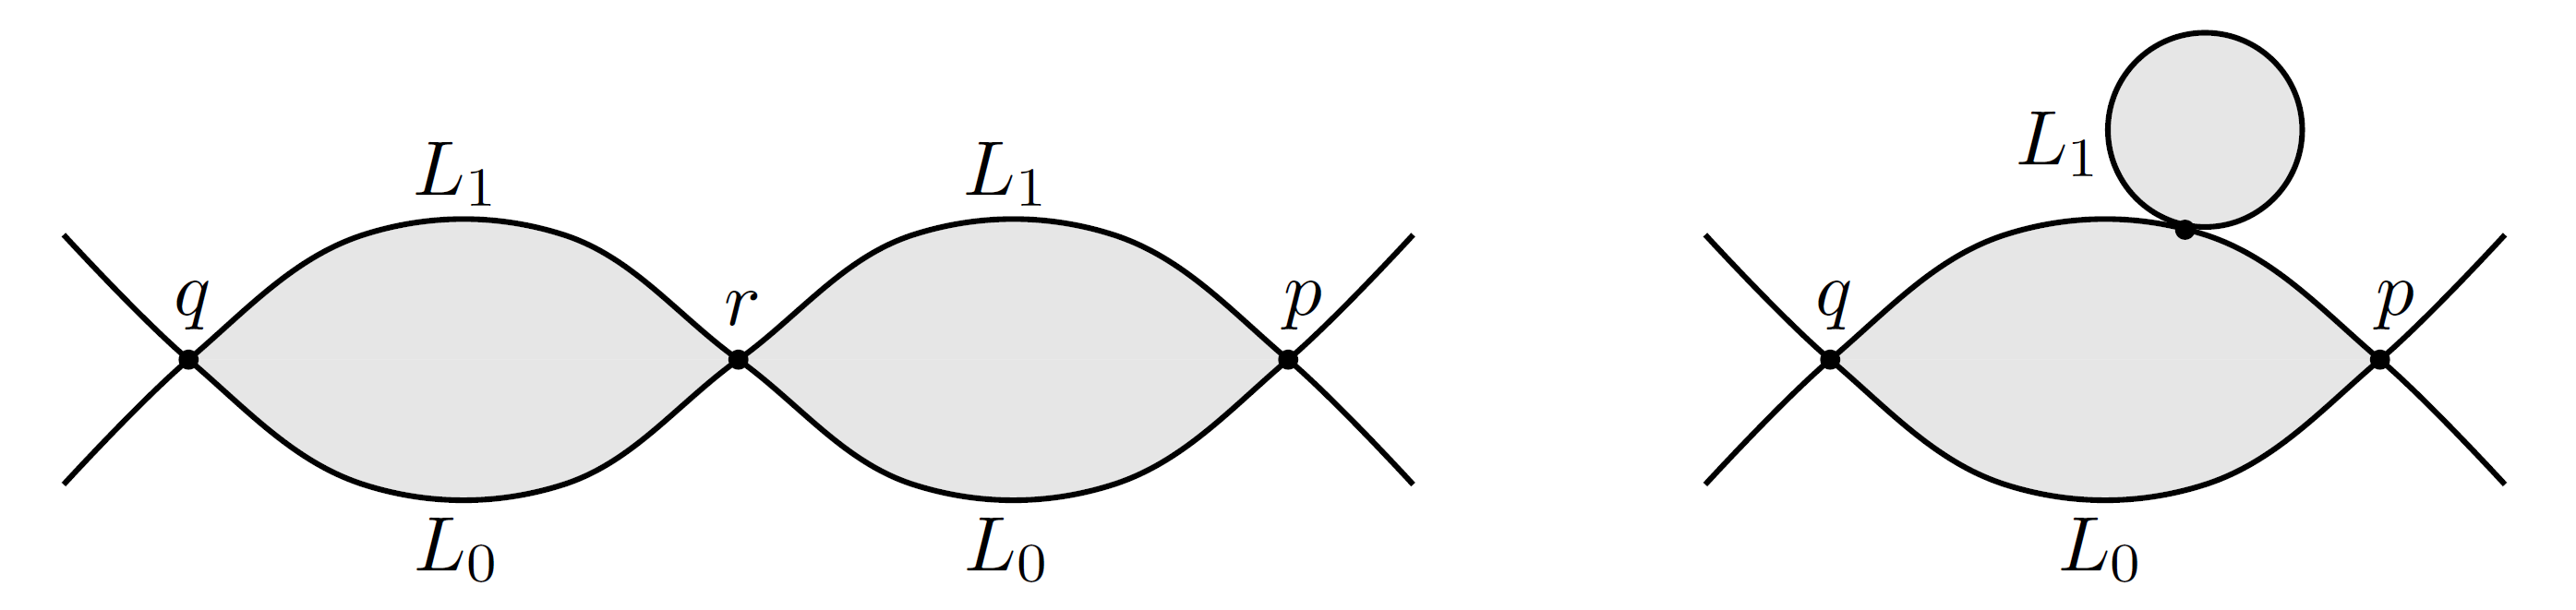
\includegraphics[width=0.9\linewidth]{fig03.png}
  \caption{两种可能的“冒泡”现象：条带断裂（左）与圆盘冒泡（右）。[来源：\cite{Aur13}]\hfill（原书 p.78）}
  \label{fig:03}
\end{figure}

这只需要求相应的 $J$-全纯圆盘与球面的辛面积
为零即可。

\begin{Lem}\label{lem:5.36}
设 $(M,\omega)$ 是辛流形，$L_0,L_1\subset M$ 是拉格朗日子流形，满足\footnote{注意
$\langle\omega\rangle\in H^2_{\mathrm{dR}}(M)\cong H^2(M;\mathbb R)\cong
\operatorname{Hom}(H_2(M),\mathbb R)\oplus\operatorname{Ext}(H_1(M),\mathbb R)
=\operatorname{Hom}(H_2(M),\mathbb R)$，于是把 $\pi_2(M)$ 与其在 Hurewicz 映射
$h:\pi_2(M)\to H_2(M)$ 下的像等同后，可把 $\langle\omega\rangle$ 限制到
$\pi_2(M)$。换言之，我们要求上同调与同调之间的配对
$\langle\langle\omega\rangle,h(\,\cdot\,)\rangle\equiv\langle\omega\rangle\cdot
\operatorname{im}(h)$ 消没，记号即由此而来。把 $\langle\omega\rangle$ 看作
$H^2_{\mathrm{dR}}(M,L_i)$ 的元素时同理。}
$\langle\omega\rangle\cdot\pi_2(M,L_i)=0$。则 $L_0$ 与 $L_1$ 不界定任何
$J$-全纯圆盘或球面。
\end{Lem}

% [Tutor Note: 【含糊】证明只有一行：若 $v:\mathbb D^2\to M$ 是边界落在 $L_i$
% 上的 $J$-全纯圆盘，则 $E(v)=\langle\omega,[v]\rangle=0$，故 $v$ 常值；球面
% 同理（因 $\pi_2(M)\to\pi_2(M,L_i)$）。原文未写出这一步，而它正是“面积为零”
% 与“无冒泡”等价的直观来源。]

这只是若干防止圆盘冒泡与球面冒泡的条件之一。后文将看到，在正合辛流形上，这一点
自动成立。

\medskip
\noindent\fbox{\parbox{0.96\linewidth}{%
此后，我们假定所有拉格朗日子流形 $L\subset M$ 都满足“无冒泡”条件
$\langle\omega\rangle\cdot\pi_2(M,L)=0$。}}
\medskip

\subsection{Floer 微分与 Floer 上同调}\label{sec:5.7}

我们终于收集齐了使后续理论适定的全部必要假设。下面着手定义 Floer 复形的第二份
数据。

\begin{Def}\label{def:5.37}
设 $(M,\omega)$ 是辛流形，$L_0,L_1\subset M$ 是拉格朗日子流形，相应的 Floer
复形 $CF(L_0,L_1)\equiv CF(L_0,L_1;J,H)$ 如 (56) 所定义（其中
$\mathcal X(L_0,L_1)=L_0\cap(\phi_H^1)^{-1}(L_1)$）。\emph{Floer 微分}
$\partial\equiv\partial_{J,H}:CF(L_0,L_1)\to CF(L_0,L_1)$ 是下式的
$\Lambda_{\mathbb K}$-线性延拓：
\begin{equation}
\partial(p):=\sum_{\substack{q\in\mathcal X(L_0,L_1)\\
[u]:\operatorname{ind}([u])=1}}
\left(\#\mathcal M(p,q;[u],J,H)\right)T^{\omega([u])}q,
\label{eq:5.74}
\end{equation}
其中 $\#\mathcal M(p,q;[u],J,H)\in\mathbb Z$（或 $\mathbb Z_2$）是来自微扰
Cauchy--Riemann 问题 (66) 的模空间 $\mathcal M(p,q;[u],J,H)$ 的（带符号或无符号）
基数，而 $\omega([u])$ 是辛面积（由无冒泡条件，它与代表元的选取无关）。由
推论 5.23，$\partial$ 的次数为 $1$。（注意 $\partial(p)$ 中 $q$ 的系数
\[
\sum_{[u]:\,\operatorname{ind}([u])=1}
\left(\#\mathcal M(p,q;[u],J,H)\right)T^{\omega([u])}\in\Lambda_{\mathbb K}
\]
是 Novikov 域的一个元素。）
\end{Def}

% [Tutor Note: 【易错】(74) 中 $T^{\omega([u])}$ 良定义依赖无冒泡条件：若
% $[u]$ 与 $[u']$ 同伦，则 $\omega([u])-\omega([u'])$ 是球面或带边圆盘的
% 面积，按假设为零。带符号计数 $\#\mathcal M$ 要求模空间可定向（定义 5.13 的
% 自旋结构），且 $\partial$ 提升次数 $+1$ 正是推论 5.23 的
% $\operatorname{ind}=\deg(q)-\deg(p)$。]

为证明 $\partial$ 良定义，还需要流形理论的最后一个（非平凡）结果。

\begin{Lem}\label{lem:5.38}
任意紧致 $1$ 维光滑流形 $M$ 的边界点的带符号总数等于零。
\end{Lem}

\begin{proof}
（略证）这是紧致 $1$ 维光滑流形分类定理的推论：任何这样的流形必微分同胚于有限
个闭实区间与若干 $S^1$ 拷贝的不交并。前者各有两个边界点，后者没有边界点。由于
边界点在微分同胚下保持，$M$ 有偶数个边界点。这直接证明了无符号计数的情形
（即模 $2$ 工作）。若我们关心定向、从而计入符号，仔细分析会揭示 $\partial M$ 的
带符号基数仍然相消。
\end{proof}

\begin{Thm}\label{thm:5.39}
设 $(M,\omega)$ 是辛流形，$L_0,L_1\subset M$ 是拉格朗日子流形，满足
$\langle\omega\rangle\cdot\pi_2(M,L_i)=0$（$i=0,1$）。则 $\partial$ 良定义，且
满足 $\partial^2=0$。此外，诱导的上同调群在选取时间依赖的 $J$ 与 $H$ 下
（在同构意义下）不变。
\end{Thm}

\begin{proof}
（略证）(74) 中的计数遍历所有同伦类
$[u]\in\pi_2(M,L_0\cup L_1)$，满足
$\operatorname{ind}([u])=\dim(\widehat{\mathcal M}(p,q;[u],J,H))=1$；于是相应的
模空间 $\mathcal M(p,q;[u],J,H)=\widehat{\mathcal M}(p,q;[u],J,H)/\mathbb R$
（由横截性它们是光滑流形）紧致、可定向且 $0$ 维，因而是可以带符号计数的有限集。
此外，(74) 中的和良定义，因为由 Gromov 紧致性定理，满足有限能量界 (67)、且其
模空间非空的同伦类 $[u]$ 只有有限多个。还要记得 $\mathcal X(L_0,L_1)$ 有限。

固定两个生成元 $p,q\in\mathcal X(L_0,L_1)$ 与某个 Maslov 指标为 $2$ 的
$[u]\in\pi_2(M,L_0\cup L_1)$。则
$\dim(\widehat{\mathcal M}(p,q;[u],J,H))=2$，于是光滑流形
$\mathcal M(p,q;[u],J,H)=\widehat{\mathcal M}(p,q;[u],J,H)/\mathbb R$ 是 $1$ 维的。
再次由命题 5.34，只需加入连接 $p$ 与 $q$、代表 $[u]$ 的断裂条带，便可把它紧化
为空间 $\overline{\mathcal M}(p,q;[u],J,H)$（按假设，没有陷入圆盘或球面冒泡的
风险）。相应地，其边界 $\partial\overline{\mathcal M}(p,q;[u],J,H)$ 含于形如
$\mathcal M(p,r;[u'],J,H)\times\mathcal M(r,q;[u''],J,H)$ 的模空间乘积之
不交并中，其中 $r\in CF(L_0,L_1)$ 是任意生成元，
$[u']+[u'']=[u]\in\pi_2(M,L_0\cup L_1)$（见图 3 左）。由于 Maslov 指标在条带
断裂下可加（按构造），且任何非常值条带的 Maslov 指标至少为 $1$（由横截性），
$\operatorname{ind}([u])=2$ 蕴含
$\operatorname{ind}([u'])=\operatorname{ind}([u''])=1$。反之，一个粘接定理\footnote{关于
某些有针对性的表述，可参看 \cite{Mer14} 第 8 节或 \cite{Sal97} 第 3.3 节，并思考
它们在 Morse 理论中的类比。}告诉我们，
$\overline{\mathcal M}(p,q;[u],J,H)$ 实际上是带边的 $1$ 维流形，且
\begin{equation}
\partial\overline{\mathcal M}(p,q;[u],J,H)
=\bigsqcup_{\substack{r\in\mathcal X(L_0,L_1)\\
[u']+[u'']=[u]\\
\operatorname{ind}([u'])=\operatorname{ind}([u''])=1}}
\mathcal M(p,r;[u'],J,H)\times\mathcal M(r,q;[u''],J,H),
\label{eq:5.75}
\end{equation}
其定向与各分量自然定向相容（后者来自 $L_0$ 与 $L_1$ 定向和自旋结构的隐含选取）。

由引理 5.38，紧致 $1$ 维光滑流形 $\mathcal M(p,q;[u],J,H)$ 的边界带符号基数
为零：
\[
\sum_{\substack{r\in\mathcal X(L_0,L_1)\\
[u']+[u'']=[u]\\
\operatorname{ind}([u'])=\operatorname{ind}([u''])=1}}
\left(\#\mathcal M(p,r;[u'],J,H)\right)\cdot
\left(\#\mathcal M(r,q;[u''],J,H)\right)=0.
\]
把最后一个表达式乘以 $\Lambda_{\mathbb K}$ 的形式变量 $T$、以总条带能量为权
$T^{\omega([u])}=T^{\omega([u'])+\omega([u''])}$，并对所有类
$[u]\in\pi_2(M,L_0\cup L_1)$ 求和，恰得 $\partial^2(p)$。因此 $\partial^2(p)=0$。

我们还须证明 $\partial=\partial_{J,H}$ 诱导的上同调群不依赖微扰数据 $J,H$ 的
选取。这里只给概览。\footnote{更多细节可在 \cite{Mer14} 第 9 章找到（非拉格朗日
情形）。}

取另一对 $(J',H')$。由于 $C^\infty([0,1],\mathcal J(M,\omega))$ 与
$C^\infty([0,1]\times M)$ 都道路连通，存在渐近常值道路
$\chi:\tau\in\overline{\mathbb R}\mapsto
(J(\tau),H(\tau))\in C^\infty([0,1],\mathcal J(M,\omega))\times
C^\infty([0,1]\times M)$，使得 $\chi(-\tau)=(J,H)$，且 $\chi(\tau)=(J',H')$
对所有 $\tau\ge N$ 成立，其中 $N\ge0$ 足够大。接着通过计数方程
\[
\partial_su+J_t(\tau,u)\left(\partial_tu-X_{H_t(\tau,u)}\right)=0
\]
的解来构造\emph{延拓映射}
$\Phi_\chi:CF(L_0,L_1;J,H)\to CF(L_0,L_1;J',H')$，方式如下：
$p'\in\mathcal X(L_0,L_1;H')$ 在 $F(p)$ 中的系数，是当
$s\to\pm\infty$ 时分别收敛到 $p$ 与 $p'$ 的指标 $0$ 解的带符号计数。对称地，
可定义延拓映射
$\Phi'_\chi:CF(L_0,L_1;J',H')\to CF(L_0,L_1;J,H)$。于是可以证明
$\partial_{J',H'}\circ\Phi_\chi=\Phi_\chi\circ\partial_{J,H}$ 与
$\partial_{J,H}\circ\Phi'_\chi=\Phi'_\chi\circ\partial_{J',H'}$，这意味着
$\Phi_\chi$ 与 $\Phi'_\chi$ 是互逆的链映射，从而
$\Phi'_\chi\circ\Phi_\chi$ 链同伦于
$\mathrm{id}_{CF(L_0,L_1;J,H)}$，而 $\Phi_\chi\circ\Phi'_\chi$ 链同伦于
$\mathrm{id}_{CF(L_0,L_1;J',H')}$。过渡到上同调便知
$H(\Phi_\chi):H(CF(L_0,L_1;J,H))\to H(CF(L_0,L_1;J',H'))$ 是同构，正如所求。
\end{proof}

% [Tutor Note: 【勘误】原文写 $\chi(-\tau)=(J,H)$ 且对 $\tau\ge N$ 有
% $\chi(\tau)=(J',H')$，其中 $\tau\in\overline{\mathbb R}$。按“渐近常值道路”
% 的通常含义应为：$\chi(\tau)=(J,H)$ 对 $\tau\le-N$，$\chi(\tau)=(J',H')$
% 对 $\tau\ge N$。译文照印原文，读者按此理解即可。]

% [Tutor Note: 【勘误】原文说 $p'$ 在“$F(p)$”中的系数，但 $F$ 在上下文里
% 没有定义；按文意应为延拓映射 $\Phi_\chi(p)$。译文照印 $F(p)$，读者按
% $\Phi_\chi(p)$ 理解即可。]

\begin{Def}\label{def:5.40}
设 $(M,\omega)$ 是辛流形，$L_0,L_1\subset M$ 是拉格朗日子流形，满足
$\langle\omega\rangle\cdot\pi_2(M,L_i)=0$（$i=0,1$）。则称
\begin{equation}
HF(L_0,L_1):=H(CF(L_0,L_1),\partial)=\frac{\ker(\partial)}
{\operatorname{im}(\partial)}
\label{eq:5.76}
\end{equation}
为\emph{拉格朗日 Floer 上同调}（由定理 5.39，可无歧义地选取任意
$J\in C^\infty([0,1],\mathcal J(M,\omega))$ 与 $H\in C^\infty([0,1]\times M)$
来定义 $CF(L_0,L_1)$ 与 $\partial$）。显式地，第 $n$ 个群为
$HF^n(L_0,L_1)=\ker(\partial_n)/\operatorname{im}(\partial_{n-1})$。
\end{Def}

由第 5.5 节的构造与定理 5.39 的证明立即推出：哈密顿同痕的拉格朗日子流形
$L_1,L_1'\subset M$ 在 Floer 上同调上诱导同构
$HF(L_0,L_1)\cong HF(L_0,L_1')$。另一方面，若 $L_0\cap L_1=\varnothing$，则
$HF(L_0,L_1)=\{0\}$。

\begin{Rem}\label{rem:5.41}
为得到 Floer \emph{同调}，必须把此前所有构造“反着”看。例如图 2 的条带从
$q$ 走向 $p$，最终导致所有分次反转。

回到上同调：在适当选取数据 $(J,H)$ 后，可以证明 Floer 复形
$CF(L_0,L_1)$ 与 $CF(L_1,L_0)$ 连同它们的微分互为对偶（此时从 $q$ 到 $p$ 的
条带是后者的一个元素）。
\end{Rem}

% [Tutor Note: 【易错】“上同调”与“同调”的差别不只是记法：把条带方向、端点
% 与 Maslov 指标同时反号后，$\partial$ 的次数从 $+1$ 变成 $-1$。原文的
% $HF(L_0,L_1)$ 是上同调，$\partial$ 提升次数；若按同调书写，需把整个复形
% 的指标取负，这正是注 5.41 所说“所有分次反转”。]

\begin{Ex}\label{ex:5.42}
看看放弃假设 $\langle\omega\rangle\cdot\pi_2(M,L_i)=0$ 会出什么问题，是有
启发性的；也就是说，允许拉格朗日子流形界定 $J$-全纯圆盘与球面。考虑 $2$ 维
流形 $M:=\mathbb R\times S^1$，带标准面积形式 $\omega:=ds\wedge dt$，以及
图 4 左所示的拉格朗日子流形 $L_0,L_1$。则 $L_0$ 与 $L_1$ 界定两张 Maslov
指标为 $1$ 的 $J$-全纯条带 $u,v$，它们分别从 $p$ 到 $q$、从 $q$ 到 $p$。按
定义，$\partial(p)=\pm T^{\omega([u])}q$ 且
$\partial(q)=\pm T^{\omega([v])}p$，于是
$\partial^2(p)=\pm T^{\omega([u])+\omega([v])}p\neq0$。
\end{Ex}

\begin{figure}[htbp]
  \centering
  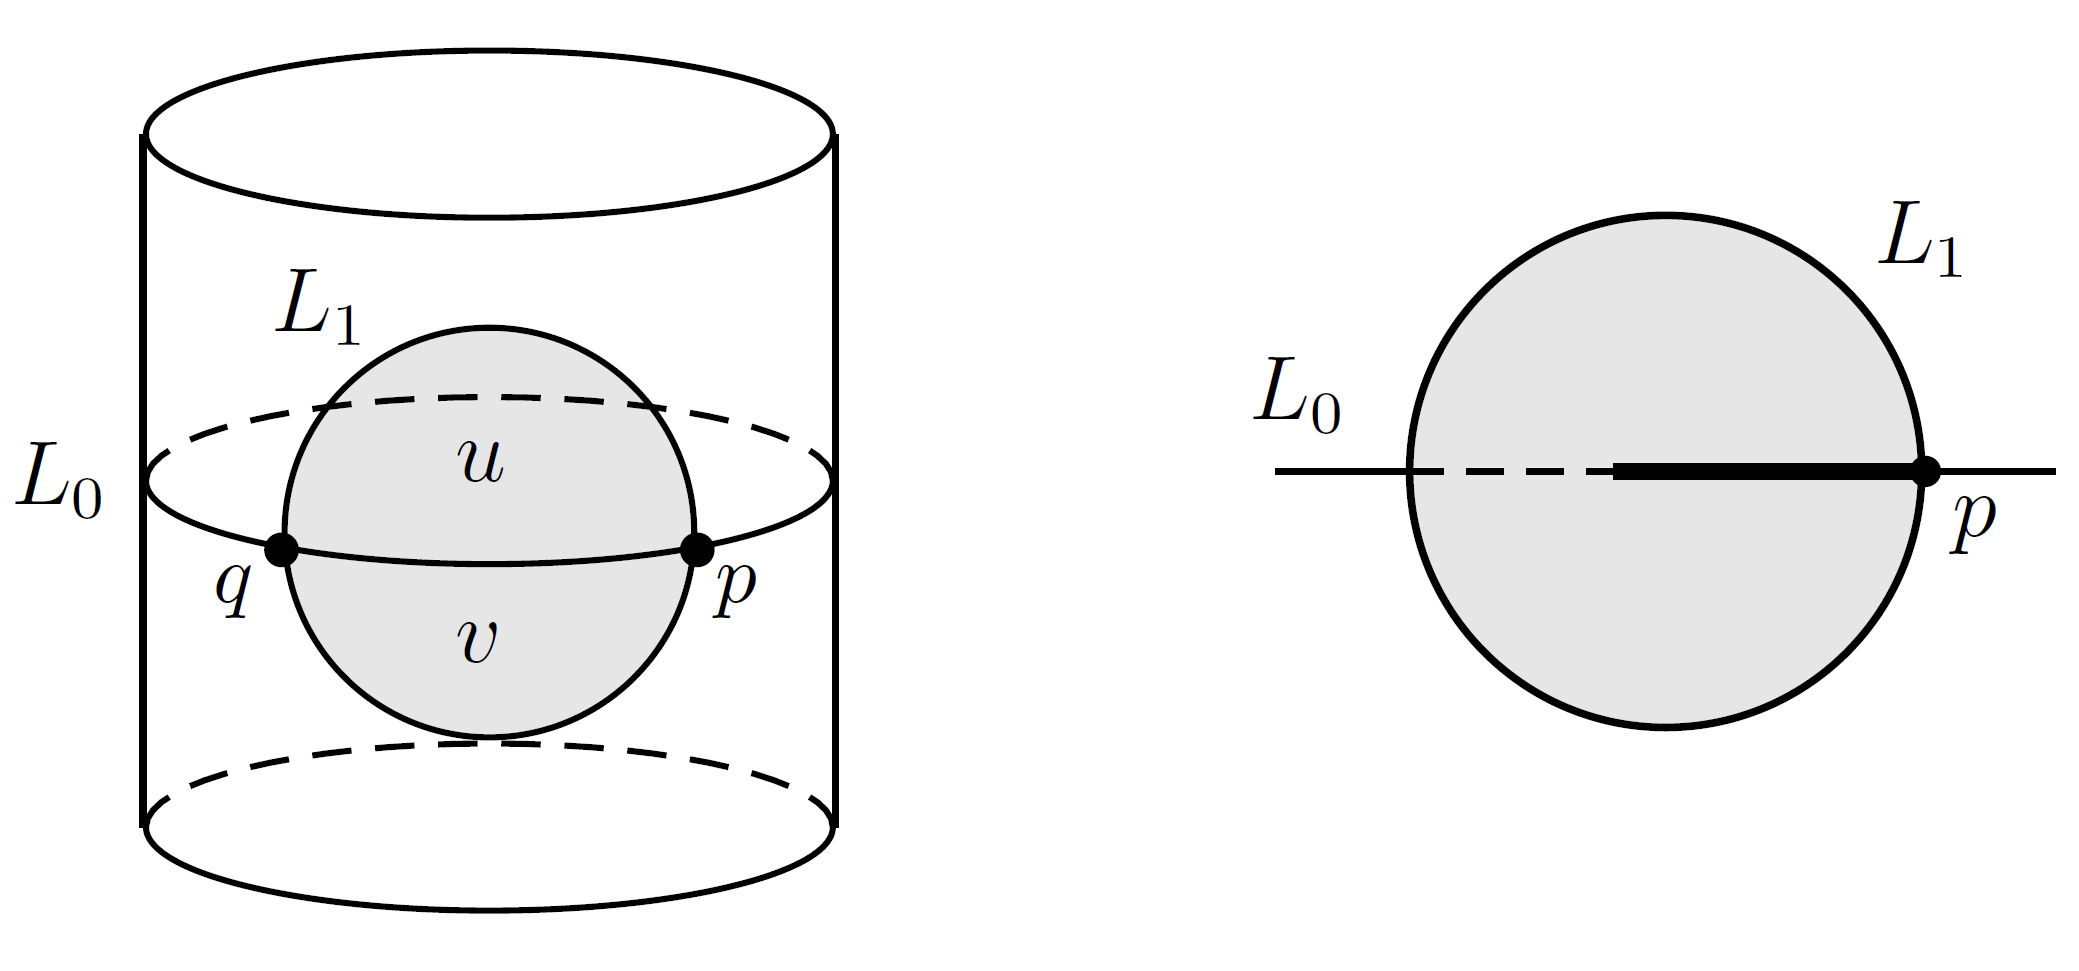
\includegraphics[width=0.8\linewidth]{fig04.png}
  \caption{若拉格朗日子流形上存在 $J$-全纯圆盘，则 Floer 微分不再平方为零。[来源：\cite{Aur13}]\hfill（原书 p.81）}
  \label{fig:04}
\end{figure}

从代数上看发生了什么？看图 4 右中 $M$ 的局部图像，在把
$\mathbb R\times[0,1]\simeq\mathbb D^2\setminus\{\pm1\}\subset\mathbb C$ 等同
之后，$L_0\supset[-1,1]$ 落在 $\mathbb R$ 上，而 $L_1$ 与 $S^1$ 重合。聚焦于
从 $p$ 到自身的指标 $2$ 的 $J$-全纯条带模空间，其像可通过沿 $L_0$（图中粗线）
剪开一条缝得到。任何这样的条带由
\[
w_\alpha(z):=\frac{z^2+\alpha}{1+\alpha z^2},
\qquad\text{其中}\quad
dw_\alpha(z)=2z\,\frac{1-\alpha^2}{(1+\alpha z^2)^2},
\]
给出，$\alpha\in(-1,1)$ 调节缝长。有两种极限情形：
\begin{itemize}
  \item 若 $\alpha\to-1$，指标 $2$ 的条带 $(w_\alpha)_\alpha$ 收敛到断裂条带
  $w$，其指标 $1$ 的分量为 $u$ 与 $v$，正如 图 3 左（确实，我们可以沿缝把
  图 4 的圆盘“打开”，并微分同胚地映为断裂构型）。这意味着能量集中在
  $z=\pm1$，正如以下所确认：
  \[
  \lim_{\alpha\to-1}|dw_\alpha(\pm1)|
  =\lim_{\alpha\to-1}\left|\frac{-4\alpha}{2(1+\alpha)}\right|=\infty.
  \]
  \item 若 $\alpha\to1$，$(w_\alpha)_\alpha$ 收敛到 $p$ 处的常值条带，并在
  $z=i$ 处带一个圆盘气泡，映到 $L_1$ 所围成的圆盘。于是能量集中在 $i$：
  \[
  \lim_{\alpha\to1}|dw_\alpha(i)|
  =\lim_{\alpha\to1}\left|\frac{4\alpha}{2(1-\alpha)}\right|=\infty.
  \]
\end{itemize}
$\alpha\to1$ 时发生的圆盘冒泡导致 $\partial^2(p)\neq0$！
\hfill$\blacklozenge$

% [Tutor Note: 【勘误】直接计算给出
% $|dw_\alpha(\pm1)|=2(1-\alpha)/(1+\alpha)$、
% $|dw_\alpha(i)|=2(1+\alpha)/(1-\alpha)$，而原文两式
% $\left|-4\alpha/(2(1+\alpha))\right|$、$\left|4\alpha/(2(1-\alpha))\right|$
% 与它们相差一个因子 $2$（且前者符号不同）。两式都仍趋于 $\infty$，故
% “能量集中”的结论不受影响；译文照印原文。]

% [Tutor Note: 【背景】例 5.42 说明：圆盘冒泡使 $\partial^2\neq0$，Floer 上
% 同调在一般辛流形上并非总是定义良好，除非引入 Kuranishi 结构/虚拟技术
% （\cite{FOOO09}）。这正是第 5.8 节转向正合流形、以及第 6 章引入 wrapped
% Fukaya 范畴的动机之一。]

最后，描述 $L_0=L_1$ 情形的 Floer 上同调。同样，以下陈述的证明对我们这个层次
来说相当高级——它涉及 Morse 理论——因此只给略证，并把读者引向 \cite{Aur13}
例 1.12。

\begin{Pro}\label{prop:5.43}
设 $(M^{2n},\omega)$ 是辛流形，$L^n\subset M$ 是拉格朗日子流形，满足
$\langle\omega\rangle\cdot\pi_2(M,L)=0$。则
$HF(L,L)\cong H(L;\Lambda_{\mathbb K})$（系数在 Novikov 域中的奇异上同调）。
\end{Pro}

\begin{proof}
（略证）首先，设 $L$ 是任意紧致实 $n$ 维流形。已知\footnote{由 Weinstein
拉格朗日邻域定理；见 \cite{Sil12} 定理 8.4。}$L\subset M$ 的某个邻域辛同胚于
$L_0:=\mathbf o(L)\subset T^*L$ 的某个邻域，其中
$\mathbf o\in\Gamma(L,T^*L)$ 表示零截面，而
$T^*L=(T^*L,\theta=\sum_i dq_i\wedge dp_i)$ 是 $L$ 的余切丛。取 Morse 函数
$f\in C^\infty(L)$ 与某个 $\varepsilon>0$，令
$L_1:=\operatorname{graph}(\varepsilon df)
=\{(x,\varepsilon(df)_x)\in T_x^*L\mid x\in L\}$。则
$L_0,L_1\subset T^*L$ 是哈密顿同痕的正合拉格朗日子流形，在
$\operatorname{crit}(f)$（即 $f$ 的临界点集）处横截相交。

选取分次提升，得到分次 Floer 复形 $CF(L_0,L_1)$，其生成元为任意
$p\in\operatorname{crit}(f)$，且 $\deg(p)=n-i(p)$（$i(p)$ 为 $p$ 的 Morse
指标）。经过适当的微扰与重标度，可以证明
$HF(L_0,L_1)\cong HM(f;\Lambda_{\mathbb K})$，即 $L$ 的 Morse 上同调，而后者
又同构于通常的奇异上同调 $H(L;\Lambda_{\mathbb K})$。连同哈密顿同痕下的不变性，
便得 $HF(L,L)\cong HF(L_0,L_0)\cong HF(L_0,L_1)\cong H(L;\Lambda_{\mathbb K})$。

现在设 $L^n\subset M$ 是满足 $\langle\omega\rangle\cdot\pi_2(M,L)=0$ 的
拉格朗日子流形。对足够小的微扰哈密顿量，决定 $HF(L,L)$ 的任何 $J$-全纯条带
必含于 $L$ 的某个小管状邻域中（由于能量约束）。因此上述分析也适用于这一般
情形。
\end{proof}

% [Tutor Note: 【勘误】原文把余切丛写成
% $T^*L=(T^*L,\theta=\sum_i dq_i\wedge dp_i)$；但 $\theta$ 应是一次形式
% （Liouville 形式 $\theta=\sum_i p_i\,dq_i$），而 $\sum_i dq_i\wedge dp_i$
% 是辛形式 $\omega_{T^*L}$（二次形式）。疑为笔误。译文照印原文；读者应以
% $\theta=\sum_i p_i\,dq_i$、$\omega=-d\theta=\sum_i dq_i\wedge dp_i$ 为准。]

% [Tutor Note: 【易错】$\deg(p)=n-i(p)$ 中 $i(p)$ 是 Morse 指标（负特征值
% 个数），故临界点的次数与 Morse 上同调的次数一致；若改用 Morse 同调（把
% 指标当作次数），所有次数变成 $i(p)$，与推论 5.23 的次数相差 $n$ 的平移。
% 这一平移是 $L$ 的分次提升选取的一部分，不影响 $HF(L,L)\cong H(L;\Lambda)$
% 的结论。]

% [Tutor Note: 【含糊】“经过适当的微扰与重标度”一句省略了关键步骤：需要把
% 条带方程在 $L$ 的管状邻域内展开，并证明只在 $\operatorname{crit}(f)$ 附近
% 有解（能量限制在小常数以下），从而把 Floer 微分与 Morse 微分逐项等同；
% 细节见 \cite{Aur13} 例 1.12 与 \cite{Sei08} 第 17 章。原文只说“可以证明”。]

再次强调，无冒泡假设 $\langle\omega\rangle\cdot\pi_2(M,L)=0$ 是本质的：否则
$HF(L,L)$（只要它有定义）可能只是 $H(L;\Lambda_{\mathbb K})$ 的一个更小的子群。

\subsection{正合流形情形}\label{sec:5.8}

在继续之前，让我们在正合辛流形 $M$ 中存在正合拉格朗日子流形 $L$ 的情形下，
简要重访上一节的理论。和以前一样，假定 $2c_1(TM)=0$，且所有 $L$ 都是紧致、
可定向、自旋、分次的，并具有消没的 Maslov 类。

\begin{Lem}\label{lem:5.44}
设 $(M^{2n},\omega)$ 是正合辛流形，$L_0,L_1\subset M$ 是正合拉格朗日子流形。
则定义 $CF(L_0,L_1)$ 的任何 $J$-全纯条带的能量为常数。此外，圆盘冒泡与球面
冒泡现象不会发生（即使我们不要求 $\langle\omega\rangle\cdot\pi_2(M,L_i)=0$！）。
\end{Lem}

\begin{proof}
设 $\omega=d\nu\in\Omega^2(M)$ 是附着于 $M$ 的正合形式，其中
$\nu\in\Omega^1(M)$；并设 $f_i\in C^\infty(L_i)$ 满足
$\nu|_{L_i}=df_i\in\Omega^1(L_i)$（$i=0,1$，参看定义 5.2）。考虑从 $p$ 到
$q$、边界在 $L_0\cup L_1$ 中的 $J$-全纯条带 $u:\mathbb R\times[0,1]\to M$，
如图 2 所示。其能量为
\begin{equation}
\begin{aligned}
E(u)&=\int_{\mathbb R\times[0,1]}u^*\omega
=\int_{\mathbb R\times[0,1]}d(u^*\nu)
&&\text{（因 $d$ 与拉回可交换）}\\
&=\int_{\partial(\mathbb R\times[0,1])}u^*\nu
&&\text{（由 Stokes 定理）}\\
&=\int_{\mathbb R\times\{1\}}u^*(\nu|_{L_1})
-\int_{\mathbb R\times\{0\}}u^*(\nu|_{L_0})
&&\text{（因 $\mathbb R\times\{i\}$ 映入 $L_i$）}\\
&=\int_{\mathbb R\times\{1\}}d(u^*f_1)
-\int_{\mathbb R\times\{0\}}d(u^*f_0)
&&\text{（因 $d$ 与拉回可交换）}\\
&=\int_{\partial(\mathbb R\times\{1\})}f_1\circ u
-\int_{\partial(\mathbb R\times\{0\})}f_0\circ u
&&\text{（由 Stokes 定理与 $u^*$ 的定义）}\\
&=\left.f_1(u(\,\cdot\,,1))\right|_{+\infty}^{-\infty}
-\left.f_0(u(\,\cdot\,,0))\right|_{+\infty}^{-\infty}
&&\text{（因我们从 $p$ 积分到 $q$）}\\
&=(f_1(q)-f_1(p))-(f_0(q)-f_0(p)).
\end{aligned}
\label{eq:5.77}
\end{equation}
因此 $u$ 的能量为常数，正如所断言。

现在考虑可能的冒泡现象。若 $v:\mathbb D^2\to M$ 是 $J$-全纯圆盘，其像在
某点 $r\in L_1$ 处与 $u$ 相交（见图 3 右），则其能量为
\[
E(v)=\int_{\mathbb D^2}v^*\omega=\int_{S^1}v^*\nu
=\int_{\partial S^1}v^*f_1=0
\]
（利用 $d$ 与 $v^*$ 可交换、两次使用 Stokes 定理，以及
$\partial S^1=\varnothing$）。类似地，设 $w:\mathbb C P^1\simeq S^2\to M$ 是
$J$-全纯球面，在某个内点处与 $u$ 相交。相应能量为
\[
E(w)=\int_{S^2}w^*\omega=\int_{\partial S^2}w^*\nu=0
\]
（因 $\partial S^2=\varnothing$）。由此可见，在两种情形下，条带的任何区域都
没有奇异的能量集中。因此圆盘冒泡与球面冒泡被排除。
\end{proof}

% [Tutor Note: 【易错】计算 (77) 时，$\partial(\mathbb R\times[0,1])$ 的
% 定向为 $\mathbb R\times\{1\}$ 取正向、$\mathbb R\times\{0\}$ 取负向，故
% 第三行两项符号相反；而 $u(+\infty)=p$、$u(-\infty)=q$，所以
% $f_1(u)|^{+\infty}_{-\infty}$ 的上限是 $+\infty$、下限是 $-\infty$。原文
% 写成 $|^{+\infty}_{-\infty}$ 却得 $f_1(q)-f_1(p)$，是因为其竖线记号的
% 上下限顺序与常规相反；译文照印，计算以 (77) 末行为准。]

% [Tutor Note: 【易错】(77) 末行不一定是正数：$E(u)\ge0$ 给出
% $(f_1(q)-f_1(p))\ge(f_0(q)-f_0(p))$，即 $f_1-f_0$ 沿条带从 $p$ 到 $q$
% 不增。这一单调性与 $E(u)=A_H(\gamma_-)-A_H(\gamma_+)$ 一致，也是
% “正合情形无冒泡”的真正原因：任何非定常圆盘或球面的能量必为零。]

因此，若与正合拉格朗日子流形打交道，使 Floer 微分良定义所需的紧致性便自动
获得。不过，若 $M$ 非紧，则需对其加一个额外假设（具体地说，$M$ 必须在无穷远
处凸，或者几何有界；例如参看 \cite{CGK02}）。又，借助方程 (77)——它告诉我们
所有辛面积都相等——可用因子 $T^{f_1(p)-f_0(p)}$ 重标度生成元
$p\in\mathcal X(L_0,L_1)$，从而 (74) 中的权重 $T^{\omega([u])}$ 可被忽略，允许
我们直接在域 $\mathbb K$ 上工作。

% [Tutor Note: 【易错】重标度的具体做法是：把生成元 $p$ 换成
% $T^{f_1(p)-f_0(p)}p$，则 (74) 中 $q$ 的系数变为
% $T^{\omega([u])+f_1(q)-f_0(q)}$；由 (77)，
% $\omega([u])=f_1(q)-f_1(p)-f_0(q)+f_0(p)$，故该指数恰为
% $f_1(p)-f_0(p)$，与 $p,q$ 之外的量无关，可整体提出。这样 $\partial$ 与
% 原来的只差一个对角共轭，上同调不变。]

最重要的是，引理 5.44 告诉我们，正合拉格朗日子流形不可能被阻碍，于是其中每
一个都是 Fukaya 范畴的（非零）对象。下面总结这一情形。

\begin{Def}\label{def:5.45}
设 $(M,\omega)$ 是正合辛流形，配有某个
$J\in C^\infty([0,1],\mathcal J(M,\omega))$ 与
$H\in C^\infty([0,1]\times M)$。设 $L_0,L_1\subset M$ 是正合拉格朗日子流形
（带有上文列出的全部数据）。$(L_0,L_1)$ 的 \emph{Floer 复形}是自由模
\[
CF(L_0,L_1)\equiv CF(L_0,L_1;H):=
\bigoplus_{p\in L_0\cap(\phi_H^1)^{-1}(L_1)}\mathbb K\cdot p,
\]
连同边界算子 $\partial\equiv\partial_{J,H}:CF(L_0,L_1)\to CF(L_0,L_1)$；后者
定义为下式的 $\mathbb K$-线性延拓：
\[
\partial(p):=\sum_{\substack{q\in L_0\cap(\phi_H^1)^{-1}(L_1)\\
[u]:\operatorname{ind}([u])=1}}
\left(\#\mathcal M(p,q;[u],J,H)\right)q
\]
（若希望忽略定向，只需作替换 $\mathbb K\leftarrow\mathbb Z_2$ 与
$\#\mathcal M(p,q;[u],J,H)\leftarrow
|\mathcal M(p,q;[u],J,H)|\ (\mathrm{mod}\ 2)$）。我们得到拉格朗日 Floer 上同调
$HF(L_0,L_1):=H(CF(L_0,L_1;H),\partial_{J,H})$；由定理 5.39 知它与
$(J,H)$ 的选取无关。
\end{Def}


